\documentclass[titlepage]{article}
\usepackage{amsmath}
\usepackage{amssymb}
\usepackage{indentfirst}
\usepackage[margin=1in]{geometry}
\usepackage{longtable}
\usepackage{enumitem}
\usepackage{fancyvrb}
%\usepackage{graphicx}
\usepackage{pdfpages}
\usepackage{subcaption}
\usepackage{flafter}
\usepackage[section]{placeins}
\usepackage{float}
\hyphenation{wave-guide}
\renewcommand\_{\textunderscore\linebreak[1]}
\setlength{\skip\footins}{10mm}

\begin{document}

\begin{titlepage}

   \centering
   \vspace*{3cm}
   {\huge\bfseries OpenParEM3D Theory, Methodology, and Accuracy} \\
   \vskip1cm
   {\Large Version 2.0} \\
   \vskip1cm
   {\Large March 2025} \\
   \vskip1cm
   {\Large Brian Young} \\

   \vfill

   \includegraphics[width=0.5\textwidth]{figures/logo-crop}

   \vspace*{\fill}
   Copyright \copyright{} 2025 Brian Young. All Rights Reserved.
\end{titlepage}

\tableofcontents

\newpage
\section{Introduction}

OpenParEM3D is a full-wave electromagnetic solver using the finite-element method to solve for frequency-dependent S-parameters and fields.  The Galerkin procedure is applied to Maxwell's equations to derive the weak form of the wave equation in the electric field $\overline{E}$.  The integrals are calculated with calls to the MFEM library \cite{MFEM}\cite{MFEMweb}, boundary conditions are applied, and finally a standard $\overline{\overline{A}}\,\overline{x}=\overline{b}$ linear problem is solved for $\overline{E}$.  Post-processing produces the magnetic field $\overline{H}$, S-parameters, and additionally for antennas far-fields, gain, directivity, and radiation efficiency.  The methodology uses fully populated matrices, so OpenParEM3D is not configured for GPU processing.

Boundary conditions include perfect magnetic conductor (PMC), perfect electric conductor (PEC), surface impedance, radiation, and 2D ports.  The 2D ports are assumed to be driven by transmission lines or waveguides, generally referred to as wave ports, so OpenParEM2D is used to calculate the 2D fields in setting up the boundary value problem.

This document covers the theory and methodology of how OpenParEM3D builds and solves the fields, S-parameters, and antenna metrics and provides the results of test cases demonstrating accuracy.  For details about how to set up and run OpenParEM3D, see the separate document "OpenParEM3D\_Users\_Manual.pdf".

\section{Theory and Mapping to MFEM}

\subsection{Wave Equation}

Starting at the most fundamental level with Maxwell's equations, we have
\begin{equation}
\label{eq:faraday}
\nabla\times\overline{E}=-\text{j}\omega\mu\overline{H}
\end{equation}
and
\begin{equation}
\label{eq:ampere}
\nabla\times\overline{H}=\overline{J}+\text{j}\omega\epsilon\overline{E}.
\end{equation}
Let $\overline{J}=\sigma\overline{E}$ and $\epsilon_c=\frac{\sigma}{\text{j}\omega}+\epsilon$, then (\ref{eq:ampere}) becomes
\begin{equation}
\label{eq:ampere2}
\nabla\times\overline{H}=\text{j}\omega\epsilon_c\overline{E}.
\end{equation}
Eliminating $\overline{H}$ from (\ref{eq:ampere2}) and (\ref{eq:faraday}) yields 
\begin{equation}
\nabla\times(-\frac{1}{\text{j}\omega\mu}\nabla\times\overline{E})=\text{j}\omega\epsilon_c\overline{E}.
\end{equation}
Multiply through by $\text{j}\omega\mu_\circ$ and set $k_\circ^2=\omega^2\mu_\circ\epsilon_\circ$ to get the wave equation
\begin{equation}
\label{eq:wave_equation}
\nabla\times(\frac{1}{\mu_r}\nabla\times\overline{E})=k_\circ^2\epsilon_{cr}\overline{E},
\end{equation}
where $\epsilon_{cr}=\epsilon_c/\epsilon_\circ$ and $\mu_r=\mu/\mu_\circ$.

\subsection{Galerkin's Procedure}

Multiply (\ref{eq:wave_equation}) by a test field $\overline{T}$ and integrate over the volume, $\Omega$, to get 
\begin{equation}
\iiint_{\Omega}\nabla\times(\frac{1}{\mu_r}\nabla\times\overline{E})\cdot\overline{T}dV=\iiint_{\Omega} k_\circ^2\epsilon_{cr}\overline{E}\cdot\overline{T}dV.
\end{equation}
The surface of $\Omega$ is designated by $\delta$.  Conventionally, the normal to the volume at the surface is given by $\hat{n}$, which points out of the 3D volume.  Apply the vector identity
\begin{equation}
\iiint_{\Omega}\nabla\times\overline{u}\cdot\overline{v}\,d\Omega=\iiint_{\Omega}\overline{u}\cdot\nabla\times\overline{v}\,d\Omega-\iint_{\delta}(\overline{u}\times\hat{n})\cdot\overline{v}\,dS
\end{equation}
with $\overline{u}=\frac{1}{\mu_r}\nabla\times\overline{E}$ and $\overline{v}=\overline{T}$ and rearranging, then
\begin{equation}
\iiint_{\Omega}\frac{1}{\mu_r}\nabla\times\overline{E}\cdot\nabla\times\overline{T}\,dV-k_\circ^2\iiint_{\Omega}\epsilon_{cr}\overline{E}\cdot\overline{T}dV-\iint_{\delta}(\frac{1}{\mu_r}\nabla\times\overline{E}\times\hat{n})\cdot\overline{T}\,dS=0.
\end{equation}
Reorder the cross products involving $\hat{n}$ to get the weak form of the wave equation in $\overline{E}$ as
\begin{equation}
\label{eq:weak_form}
\iiint_{\Omega}\frac{1}{\mu_r}\nabla\times\overline{E}\cdot\nabla\times\overline{T}\,dV-k_\circ^2\iiint_{\Omega}\epsilon_{cr}\overline{E}\cdot\overline{T}dV+\iint_{\delta}\hat{n}\times(\frac{1}{\mu_r}\nabla\times\overline{E})\cdot\overline{T}\,dS=0.
\end{equation}

In (\ref{eq:weak_form}) the first two terms are volume integrals over the entire simulation domain, while the third term is a surface integral over the outer surface of the simulation domain and represents the boundary conditions that must be applied to obtain a unique solution.  Most of the work in implementing a simulator is in setting up the various components of the surface integrals.

\subsection{Boundary Conditions}

The third term in (\ref{eq:weak_form}) captures the boundary conditions, and the entire surface must be treated to produce a unique solution.  The boundary can be subdivided into areas requiring different boundary conditions as
\begin{equation}
\label{eq:boundary}
\begin{array}{rcclr}
\iint_{\delta}\hat{n}\times(\frac{1}{\mu_r}\nabla\times\overline{E})\cdot\overline{T}\,dS & = &   & \iint_{\delta_{\text{PMC}}}\hat{n}\times(\frac{1}{\mu_r}\nabla\times\overline{E})\cdot\overline{T}\,dS & \text{PMC} \\[5pt]
                                                                                          &   & + & \iint_{\delta_{\text{PEC}}}\hat{n}\times(\frac{1}{\mu_r}\nabla\times\overline{E})\cdot\overline{T}\,dS & \text{PEC} \\[5pt]
                                                                                          &   & + & \sum_{i=1}^{M_Z}\iint_{\delta_{Z_{si}}}\hat{n}\times(\frac{1}{\mu_r}\nabla\times\overline{E})\cdot\overline{T}\,dS & \text{surface impedance}\\[5pt]
                                                                                          &   & + & \sum_{i=1}^{M_R}\iint_{\delta_{R_{i}}}\hat{n}\times(\frac{1}{\mu_r}\nabla\times\overline{E})\cdot\overline{T}\,dS & \text{radiation}\\[5pt]
                                                                                          &   & + & \sum_{i=1}^{M_P}\iint_{\delta_{P_{i}}}\hat{n}\times(\frac{1}{\mu_r}\nabla\times\overline{E})\cdot\overline{T}\,dS  & \text{ports}
\end{array}
\end{equation}

\subsubsection{PMC}

The perfect magnetic conductor (PMC) from the first line of (\ref{eq:boundary}) is the easiest boundary to implement because simply nothing has to be done. The PMC boundary is the natural boundary that happens when the degrees of freedom (DOF)\footnote{A variable used to implement a finite element is referred to as a degree of freedom (DOF).  A higher-order finite element requires more DOFs than a lower-order finite element.} of the boundary are left to float.

\subsubsection{PEC}

The perfect electric conductor (PEC) from the second line of (\ref{eq:boundary}) is applied by setting the boundary DOFs of PEC boundaries to zero.  Nedelec finite elements are used for $\overline{E}$, and these only have tangential components at boundaries.  Setting the DOFs to zero at the boundary then forces the tangential component of $\overline{E}$ to zero at the boundary, satisfying the PEC boundary condition.

\subsubsection{Surface Impedance}

The third line in (\ref{eq:boundary}) implements a surface impedance $Z_{si}$ over $M_Z$ sections of the boundary. $Z_s$ relates the tangential electric and magnetic fields on the surface via
\begin{equation}
\overline{E}_t=-Z_s\,\hat{n}\times\overline{H},
\end{equation}
where $\hat{n}$ is the unit vector normal to the surface pointing out of the 3D space.  The minus sign is necessary since $\overline{E}\times\overline{H}$ points outward for power dissipation, then $-\hat{n}\times\overline{H}$ points in the direction of $\overline{E}$.  Substituting $\overline{H}$ from (\ref{eq:faraday}) yields
\begin{equation}
\overline{E}_t=\frac{Z_s}{\text{j}\omega\mu}\hat{n}\times\nabla\times\overline{E}.
\end{equation}
This can be directly substituted into the third line of (\ref{eq:boundary}) to find that
\begin{equation}
\label{eq:third_term}
\sum_{i=1}^{M_Z}\iint_{\delta_{Z_{si}}}\hat{n}\times(\frac{1}{\mu_r}\nabla\times\overline{E})\cdot\overline{T}\,dS=\sum_{i=1}^{M_Z}\iint_{\delta_{Z_{si}}} \frac{\text{j}\omega\mu_{\circ}}{Z_{si}}\overline{E}_t\cdot\overline{T}\,dS.
\end{equation}

\subsubsection{Radiation}

The fourth line in (\ref{eq:boundary}) implements a radiation boundary condition (RBC) over $M_R$ sections of the boundary.  Using a 1$^{\textnormal{st}}$-order RBC, also known as a Sommerfeld RBC, propagation is assumed in the far field to have the dependence $e^{-\text{j}kr}$ in the $\hat{n}$ radial direction, where $k$ is the propagation constant and $r$ is the radial distance from the radiating source, then  
\begin{equation}
\label{eq:rbc_term}
\hat{n}\times(\frac{1}{\mu_r}\nabla\times\overline{E})=\frac{\text{j}k}{\mu_r}\overline{E}.
\end{equation}
This can be easily demonstrated in Cartesian coordinates by working through the math with $\overline{E}=E_o e^{-jkz}\hat{x}$. Plugging (\ref{eq:rbc_term}) back into the 4$^{\textnormal{th}}$ line of (\ref{eq:boundary}) produces
\begin{equation}
\label{eq:fourth_term}
\sum_{i=1}^{M_R}\iint_{\delta_{R_{i}}}\hat{n}\times(\frac{1}{\mu_r}\nabla\times\overline{E})\cdot\overline{T}\,dS=\sum_{i=1}^{M_R}\iint_{\delta_{R_{i}}}\frac{\text{j}k}{\mu_r}\overline{E}\cdot\overline{T}\,dS.
\end{equation}

Noting the similar forms for (\ref{eq:third_term}) and (\ref{eq:fourth_term}), the equivalent "surface impedance" of the RBC can be found by equating the factors $\frac{\text{j}\omega\mu_{\circ}}{Z_{si}}$ and $\frac{\text{j}k}{\mu_r}$, then noting that $k=\omega\sqrt{\mu\epsilon}$ and simplifying results in $Z_{si}=\sqrt{\mu/\epsilon}$, which is simply the wave impedance for a plane wave.  So in short, the 1$^{\textnormal{st}}$-order RBC is equivalent to setting the boundary to a surface impedance equal to the wave impedance.

To apply the 1$^{\textnormal{st}}$-order RBC, the electromagnetic fields must be in a plane wave configuration at the boundary, with $\overline{E}$ perpendicular to $\overline{H}$ and both perpendicular to the surface.  In practical simulation setups with reasonably sized volumes, this condition will not be met with high precision.  However, it can be met with engineering precision, so it is practical for typical design work.  When the boundary is too close to the radiating structure, plots show a weak but visible standing wave at the boundary.

\subsubsection{Port}
\label{sec:port}

The fifth line in (\ref{eq:boundary}) implements ports, where energy enters and exits the 3D space as modes of transmission lines or waveguides.  Since ports are on the surface, they are 2D.  It is assumed that the fields at the ports represent transmission line or waveguide solutions with a dependence in the direction of propagation $\hat{n}$ of $e^{-\gamma n}$.  This assumption means that the ports can only be applied to planar 2D surfaces on the boundary of the 3D space.  Ports defined in this way are generally referred to as \textit{wave ports}.

A distinction must be made between ports drawn on the 3D surface and S-parameter ports.  A closed outline drawn on a planar region of the 3D surface is a physical port representing a transmission line or waveguide, which may support one or more propagating modes.  For example, a port capturing two symmetric strip transmission lines with the port boundary being set to PEC supports two modes: even and odd.  Every mode of a port becomes a column and row in the final S-parameter matrix, and so in this example one port provides two rows and columns.  The name used here to describe the row/column of the S-parameter matrix is \textit{S-parameter port} or \textit{S-port}.  For the example with two symmetric strip transmission lines, one port leads to 2 S-ports.  When there is one mode per port, then the number of ports and S-ports are equal.

To ultimately solve for the S-parameters, a port must be driven with a 2D field configuration while the remaining ports must be terminated with a 2D absorbing boundary condition (2D ABC).  So  \textit{two} boundary conditions are needed for the ports: driving and 2D ABC.

For the port boundary condition when driving, the 2D solution from OpenParEM2D is simply imposed onto the port by equating the port boundary DOFs to the values computed in OpenParEM2D.  The imposed solution may be the dominant or a higher-order mode, depending on the problem setup.  Continuing with the symmetric strip transmission line example, a port is driven once for the even mode and a second time for the odd mode.

To construct a 2D ABC, using the 5$^{\textnormal{th}}$ line of (\ref{eq:boundary}), the vector identity
\begin{equation}
\label{eq:fifth_term}
\hat{n}\times\nabla\times\overline{E}=-\frac{\partial\overline{E}_t}{\partial{n}}+\nabla_t E_n=\gamma \overline{E}_t + \nabla_t E_n,
\end{equation}
is applied, where the assumption for a propagating transmission line or waveguide mode is used such that the field dependence along the direction of travel, $\hat{n}$, is $e^{-\gamma n}$. The gradient term $\nabla_t E_n$ is not directly supported by Nedelec finite elements in MFEM and requires additional consideration.

OpenParEM3D uses Nedelec finite elements because the divergence for the elements is zero, so the two $\nabla\cdot$ terms of Maxwell's equations are satisfied and spurious (i.e. incorrect) solutions are avoided.  A Nedelec finite element contains only tangential vector terms on the faces of the element, so $\nabla_t E_n$ presents a problem in that the boundary does not have a normal component on which to make the calculation.  During a simulation, the normal component on the boundary is computed as a natural result of the 3D solution, so the simulations correctly include the normal component.  However, the MFEM library does not include a function to directly implement the needed gradient term on the boundary, perhaps due to the need to pull the needed information from multiple finite elements.

To obtain the needed gradient term, the wave equation in 3D given by (\ref{eq:wave_equation}) can be revisited in 2D at the port.  In 2D, the dependence in the direction of propagation is $e^{-\gamma n}$, and the electric field and operator can be divided into tangential and normal components as $\overline{E}=\overline{E}_t + E_n \hat{n}$ and $\nabla=\nabla_t - \gamma \hat{n}$. Applying these to (\ref{eq:wave_equation}) and equating the tangential and normal components results in two coupled equations
\begin{equation}
\label{eq:first_2D_term}
\nabla_t\times\frac{1}{\mu_r}\nabla_t\times\overline{E}_t-\gamma^2\frac{1}{\mu_r}\overline{E}_t-\gamma\frac{1}{\mu_r}\nabla_t E_n=k_{\circ}^2 \epsilon_{cr}\overline{E}_t
\end{equation}
and
\begin{equation}
\label{eq:second_2D_term}
\nabla_t\cdot\frac{1}{\mu_r}\nabla_t E_n+\frac{1}{\mu_r}\gamma\nabla_t\cdot\overline{E}_t+k_{\circ}^2\epsilon_{cr}E_n=0.
\end{equation}
The needed term from (\ref{eq:fifth_term}) can be pulled from (\ref{eq:first_2D_term}) to obtain
\begin{equation}
\label{eq:2D_ABC}
\gamma \overline{E}_t + \nabla_t E_n=\frac{1}{\gamma}(\nabla_t \times \nabla_t \times \overline{E}_t - k_{\circ}^2 \epsilon_{cr}\mu_r \overline{E}_t),
\end{equation}
and the terms on the right side of the equality are supported by MFEM since only tangential components are called for.  Plugging (\ref{eq:2D_ABC}) back into the 5$^{\textnormal{th}}$ line of (\ref{eq:boundary}) produces
\begin{equation}
\label{eq:fifth_term_final}
\sum_{i=1}^{M_P}\iint_{\delta_{P_{i}}}\hat{n}\times(\frac{1}{\mu_r}\nabla\times\overline{E})\cdot\overline{T}\,dS=\sum_{i=1}^{M_P}\iint_{\delta_{P_{i}}}\frac{1}{\gamma}(\nabla_t \times \nabla_t \times \overline{E}_t - k_{\circ}^2 \epsilon_{cr}\mu_r \overline{E}_t)\cdot\overline{T}\,dS.
\end{equation}


There is still the issue of (\ref{eq:second_2D_term}), which is not coded into the simulation. The normal components at the boundary derive their behavior from the 3D behavior of the fields near the boundary and are governed by the wave equation (\ref{eq:wave_equation}).  The general solution in 3D space then ensures that (\ref{eq:second_2D_term}) is satisfied.  It would be beneficial to numerically prove this observation, but the needed functions are not provided by the MFEM library for the reasons discussed above.  However, the accuracy demonstrations in Sec.~\ref{sec:accuracy} include an example with a $TM$ field configuration with significant $E_n$ field strength for which the 2D ABC is shown to be very effective.

There is a very important point to consider and understand with respect to (\ref{eq:fifth_term_final}): the presence of $\gamma$.  Only one value for $\gamma$ can be applied at a given port in its 2D ABC.  If there is a single propagating mode on the port, then it is matched and the 2D ABC is very effective.  If there is more than one propagating mode on the port, and the modes do not have the same $\gamma$, only one mode can be fully absorbed by the 2D ABC.  Any other modes will suffer some reflection with a reflection coefficient roughly equal to the ratio of the $\gamma$s for the modes.  For example, coupled stripline will not suffer reflections since the even and odd modes have equal $\gamma$, but coupled microstrip will suffer some reflection since the $\gamma$ for the even and odd modes are not equal.  The impact of any reflection from the 2D ABC for mismatched $\gamma$s from multiple modes may or may not be relevant to engineering applications for a given problem.  To avoid active S-parameters, at a multimode port the largest $\gamma$ is used for the 2D ABC.

\subsection{Calculating $\overline{H}$ from $\overline{E}$}

Slightly rearranging (\ref{eq:faraday}) to find an expression for $\overline{H}$ produces
\begin{equation}
\overline{H}=-\frac{1}{\text{j}\omega\mu}\nabla\times\overline{E}.
\end{equation}
Applying the Galerkin procedure by multiplying through by a weight $\overline{T}$ and integrating over the volume results in
\begin{equation}
\label{eq:Hfield}
\iiint_{\Omega}\overline{H}\cdot\overline{T}\, dV=\text{j}\iiint_{\Omega}\frac{1}{\omega\mu}\nabla\times\overline{E}\cdot\overline{T}\,dV.
\end{equation}
These volume integrals are directly supported by MFEM.  No additional boundary conditions need to be applied in addition to those applied when solving for $\overline{E}$.

\subsection{Construction and Solution of the $\overline{\overline{A}}\,\overline{x}=\overline{b}$ Problem}

The boundary value problem to be solved to find $\overline{E}$ in the 3D volume and on the boundaries is defined by (\ref{eq:weak_form}) and (\ref{eq:boundary}).  To recap, the boundary conditions are given by (\ref{eq:third_term}) for impedance, (\ref{eq:fourth_term}) for radiation, and (\ref{eq:fifth_term_final}) for 2D ABCs at ports.  The role of the MFEM library is to provide the function calls to implement each mathematical operation in these equations (volume and boundary) by using finite elements to build matrices enabling the construction of the standard numerical problem $\overline{\overline{A}}\,\overline{x}=\overline{b}$.  Additional boundary conditions are applied directly to the $\overline{\overline{A}}\,\overline{x}=\overline{b}$ problem by setting DOFs for PEC boundaries and for 2D port excitations.  Ultimately, the linear problem is solved for $\overline{x}$ given $\overline{b}$, where $\overline{x}$ are the DOFs for $\overline{E}$ and $\overline{b}$ are the boundary conditions.

MFEM is fundamentally built around real variables, while OpenParEM3D is a frequency-domain solver requiring complex variables. While there are some wrappers in MFEM to connect real data structures into complex data structures, an issue is that MFEM requires the real variable version of PETSc \cite{PETSc}.  It is possible to solve the complex $\overline{\overline{A}}\,\overline{x}=\overline{b}$ problem using real variables, but testing showed that performance is dramatically better using complex variables, which requires the complex version of PETSc. So throughout the code of OpenParEM3D, MFEM is used to construct real matrices for the real and imaginary parts of the math, and then these two real matrices are combined into complex matrices for solution with PETSc compiled for complex variables.  There is an impact on dynamic memory usage because the real and complex data structures have to be allocated at the same time before complex construction is complete and the real data structure can be deleted.  However, there is not a significant impact on run time from the data translations since the vast majority of simulation time is spent solving the complex $\overline{\overline{A}}\,\overline{x}=\overline{b}$ problem.

The construction and solution of the 3D electromagnetic problem is executed in \texttt{fem3D::solve}.  Discussion on each step follows.

\subsubsection{Building $\overline{\overline{A}}$}

With the exception of the application of the PEC boundary, construction of $\overline{\overline{A}}$ occurs in \texttt{fem2D::build\_A}. Construction involves making appropriate calls to MFEM methods to implement the needed physics in finite elements.

In solving (\ref{eq:weak_form}), the MFEM mapping of the first two integrals are
\begin{equation}
\begin{array}{lcr}
\iiint_{\Omega}\frac{1}{\mu_r}\nabla\times\overline{E}\cdot\nabla\times\overline{T}\,dV & \rightarrow & \text{CurlCurlIntegrator} \\[5pt]
k_\circ^2\iiint_{\Omega}\epsilon_{cr}\overline{E}\cdot\overline{T}dV & \rightarrow  & \text{VectorFEMassIntegrator}
\end{array}
\end{equation}
The matrix is built by MFEM as a \texttt{ParMixedBilinearForm} structure that is converted to a \texttt{HypreParMatrix} parallel matrix suitable for parallel processing using the Message Passing Interface (MPI) through the \texttt{Assemble} and \texttt{Finalize} operations.  Since the \texttt{ParMixedBilinearForm} is rendered into filled-out matrices, GPU processing is ruled out due to the large memory allocation for typical problems.  To enable GPU processing, the formulation would need to be re-structured and re-coded to avoid using filled-out matrices.

The remaining part of implementing (\ref{eq:weak_form}) involves applying the boundary conditions, with ports, surface impedance, and radiation boundary conditions applied in \texttt{fem2D::build\_A}.

For non-driving ports, port boundary conditions are applied in \texttt{Port::addPortIntegrators}. The 2D ABC boundary condition is defined in (\ref{eq:fifth_term_final}), and it is implemented in \texttt{Port::addPortIntegrators} using MFEM CurlCurlIntegrator and VectorFEMassIntegrator on the port boundaries.  Note at the top of \texttt{Port::addPortIntegrators} how $\gamma$ is selected for multimode ports. 

Impedance and radiation boundary conditions are applied in \texttt{Boundary::addImpedanceIntegrators}.  Here, the method name is appropriate because both (\ref{eq:third_term}) and (\ref{eq:fourth_term}) are implemented with an MFEM VectorFEMassIntegrator applied over the appropriate boundaries.

The final step in preparing $\overline{\overline{A}}$ in \texttt{fem3D::build\_A} is to combine the real and imaginary \texttt{HypreParMatrix}s into a PETSc complex \texttt{MAT} matrix using the \texttt{hypre\_ParCSRMatrixToMat} routine.  As the complex \texttt{MAT} is constructed, the \texttt{HypreParMatrix}s are deleted.

\subsubsection{PEC Boundary}

After the call to \texttt{fem3D::build\_A}, the next boundary condition to apply is the PEC boundary.  The first step is to identify the PEC boundary DOFs using \texttt{fem3D:build\_PEC\_dofs}, then these are used to enforce the PEC boundary by zeroing the row and column for each PEC DOF in $\overline{\overline{A}}$ while placing the number 1 on the diagonal in \texttt{eliminatePEC} from file \texttt{solveComplexLinearSystem.c}.

\subsubsection{Driving Port Boundary}

The final boundary condition to apply is the electric field from the 2D solution from OpenParEM2D at the driving port.  There are no MFEM calls associated with setting this boundary condition.  With the driving mode on the driving port identified, \texttt{Mode::fillX} fills a vector with the known boundary DOFs on the port.

\subsubsection{Solution}

The driving port DOFs and $\overline{\overline{A}}$ are passed to the function \texttt{solveComplexLinearSystem} in file \newline\texttt{solveComplexLinearSystem.c}, which builds $\overline{b}$ and solves the completed $\overline{\overline{A}}\,\overline{x}=\overline{b}$ problem using PETSc's KSP infrastructure.  Once solved for the 3D electric field DOFS, the DOFs are translated back into MFEM data structures with calls to \texttt{fem3D::build\_e\_re\_e\_im} and \texttt{fem3D::buildEgrids}.  Further plotting and post-processing for S-parameters uses the data in the MFEM ParGridFunction data structure.

\subsubsection{H Field}

OpenParEM3D uses the H-field to separate forward- and reverse- traveling waves at the ports, so it is always required to calculate the magnetic fields.  The H-field is derived from the E-field using (\ref{eq:Hfield}), which is calculated in \texttt{fem3D::buildHgrids}.  The integrals in (\ref{eq:Hfield}) are set up in \texttt{fem3D::build\_P} for the left-hand side using an MFEM VectorFEMassIntegrator, followed by conversion to complex PETSc MAT, and in \texttt{fem3D::build\_Q} for the right-hand side using an MFEM MixedVectorCurlIntegrator, also followed by conversion to complex PETSc MAT.  Since the right-hand side involves $\overline{E}$, which is known at this point, the E-field DOFs are applied to generate $\overline{b}$ for an $\overline{\overline{A}}\,\overline{x}=\overline{b}$ problem, with $\overline{\overline{A}}=\overline{\overline{P}}$, which is solved in \texttt{solveHfield} using the PETSc KSP infrastructure.

Like for the electric fields, once the H-field DOFs are known, they are translated back into MFEM data structures with a call to \texttt{fem3D::build\_h\_re\_h\_im} and construction of ParGridFunction structures which are used for S-parameter calculations and plotting.

\subsection{Far Field Calculation}

Once the solutions for the E- and H- fields are computed in the 3D solution space, post-processing is used for antennas to calculate the far-field radiation pattern and derived quantities such as directivity, gain, and efficiency.  For an antenna, the outer surfaces of the 3D space are given a radiation boundary condition.  Since OpenParEM3D supports a 1$^{\textnormal{st}}$-order radiation boundary condition, the distance between the radiation boundaries and the antenna must be a couple of wavelengths at the lowest frequency of interest to limit reflections.

\subsubsection{Surface Currents}

The first post-processing step is to calculate the electric and magnetic currents on each of the radiation boundaries.  The calculation is performed in \texttt{Boundary::calculateRadiationCurrents}.  The 3D field solutions are first transferred from the 3D finite element mesh to 2D meshes on the boundaries using MFEM's ParSubMesh functionality, then the currents are calculated on the 2D mesh as
\begin{equation}
\label{eq:J_current}
\overline{J}=\hat{n}\times\overline{E}
\end{equation}
and
\begin{equation}
\label{eq:M_current}
\overline{M}=-\hat{n}\times\overline{H},
\end{equation}
where $\hat{n}$ is the normal to the radiation boundary pointing outwards from the 3D space.  The cross product is implemented using a ParDiscreteLinearOperator with a VectorCrossProductInterpolator from the MFEM library.  Both real and imaginary parts must be calculated.

With the currents on the radiation boundaries known, in princple, the far fields can then be calculated using the far-field Green's function.  However, this calculation is not supported by the MFEM library.  To add this calculation requires a very deep understanding of finite elements, arbitrary order finite element basis functions, quadrature integration rules, discrete linear operators, and how all of these are implemented in the MFEM library.  This is a daunting task that is bypassed in OpenParEM3D for now.

Instead of precisely using $\overline{J}$ and $\overline{M}$ from the finite element representation, values of $\overline{J}$ and $\overline{M}$ are sampled on a grid with uniform spacing of $0.1\lambda$ [which is user configurable] so that the far-field calculation can proceed outside of the MFEM library.  Once the currents are sampled, then the Green's function calculation can proceed.
The ultimate product of \texttt{Boundary::calculateRadiationCurrents} are $\overline{J}$ and $\overline{M}$ sampled on a grid on the radiation boundaries and stored in the vector \texttt{radiationCurrents}.

Note that sampling the currents on a grid introduces computational inefficiency since the finite elements themselves can be large compared to the wavelength, especially for higher-order finite elements.  Since each point in the far field must sum over all currents on all radiation boundaries, the fine gridding of the currents appear in an inner loop and can become very slow.  However, \texttt{radiationCurrents} is duplicated across all ranks when parallel processing, so far-field calculations for radiation patterns are parallelizable with very high efficiency and high core counts are effective at addressing the inefficiency caused by fine sampling of the current.

\subsubsection{Far Fields}

Once the surface currents are calculated, the electromagnetic solution in the far field can be found using the far-field Green's function.  The calculation can be found in \texttt{BoundaryDatabase::calculateFarField} using the equations from \cite{Balanis}.  The calculation simply sums the far-field contribution from each current element on the radiation boundaries, where the currents are stored in \texttt{radiationCurrents}.
Far field values are calculated over one sphere and optional circles representing planar cuts through the sphere, and these are defined in the file \texttt{patterns.hpp}.

The sphere is described by triangles defined by vertex points, and the fields are calculated for each vertex.  Integrated values over the surface are calculated as the field value times the area assigned to that vertex, where the area consists of the sum of a fraction of the areas of all triangles utilizing that vertex [see \texttt{Sphere::allocateAreasToPoints}].

For circles, the starting point is a plane in x-y plane that is then rotated in spherical coordinates with $\phi$ being the angle in the x-y plane from the x-axis and $\theta$ bing the angle from the z-axis.  A plane in the x-y plane has no rotation, so $\theta=\phi=0$.  For the y-z plane, the starting x-y plane must be rotated with $\theta=90^\circ$, and for the x-z plane, $\theta=\phi=-90^\circ$.  In addition, the plane can be shifted in the direction normal to the plane using a parameter called "latitude".  For an x-y plane, the latitude is equivalent to the latitude on Earth, where $0^\circ$ is at the equator and $90^\circ$ is at the north pole.  The fields are calculated at points uniformly spaced around the circle.

\subsubsection{Accepted Power}

The antenna gain calculation requires the accepted power, which is the amount of power flowing into the driven ports. For a single driven port, the total power is $P_{\text{total}}=P_{\text{out}}-P_{\text{in}}$, where $P_{\text{out}}$ is the power reflected from the port due to impedance mismatch.  Since the impedance mismatch can always be addressed with a matching circuit, the reflected power is not an inherent property of the antenna, so $P_{\text{in}}$ forms the basis of the gain calculation.

At a given port, the power at the port is given by
\begin{equation}
P=\frac{1}{2}\iint \overline{E}_t\times\overline{H}_t^{*} dS.
\end{equation}
The total fields can be broken into directional modal fields using (\ref{eq:Et}) and (\ref{eq:Ht}).  For a one-port antenna, the power flowing into the port is then
\begin{equation}
P_\text{in}=\frac{1}{2}\iint C^{-}\overline{E}^{-}_{tm}\times C^{-*}\overline{H}^{-*}_{tm} dS
\end{equation}
Given that the modal power into the port from the 2D port simulation is
\begin{equation}
P_{z}=\frac{1}{2}\iint \overline{E}^{-}_{tm}\times\overline{H}^{-*}_{tm} dS,
\end{equation}
then the power entering the port, the accepted power, is
\begin{equation}
P_{\text{in}}=C^{-}C^{-*}P_z.
\end{equation}
The value for $P_z$ is taken from the 2D port simulation, and the value for $C^-$ is the same as that from Sec.~\ref{sec:C}, which is calculated during S-parameter extraction.
The calculation for $P_{\text{in}}$ is made in \newline\texttt{BoundaryDatabase::calculateAcceptedPower}, where the calculation is generalized for multiport antennas.

\subsubsection{Derived Quantities}

Once the sphere is populated with computed far-field values, quantities of interest for antennas can be calculated.  The isotropic gain is calculated in \texttt{Sphere::calculateIsotropicGain} and directivity is calculated in \texttt{Sphere::calculateDirectivity}.  Radiation efficiency is calculated in \newline\texttt{Pattern:calculateRadiationEfficiency}.

\section{S-parameter Calculation}

A primary engineering output from OpenParEM3D are S-parameters, which are post-processed from the computed 3D electric and magnetic fields.  Consider a black box with $N$ S-ports as shown in Fig.~\ref{fig:Sport}, where the physical ports as discussed in Sec.~\ref{sec:port} are not shown.  The S-parameters of the black box relate the outward-traveling waves $b_i$ to the inward-traveling waves $a_i$ using the S-parameter matrix as $\overline{b}=\overline{\overline{S}}\,\overline{a}$, which is shown in expanded form in (\ref{eq:Sparameters}).  The goal is to find $\overline{\overline{S}}$ from 3D electromagnetic field calculations.

\begin{figure}
  \centering
  \includegraphics[width=0.25\textwidth]{figures/Sport-crop}
  \caption{S-parameter black box with N S-parameter (S-port) ports.}
  \label{fig:Sport}
\end{figure}

\begin{equation}
\label{eq:Sparameters}
\left[ \begin{array}{c}
  b_1 \\
  b_2 \\
  \vdots \\
  b_N \\
\end{array} \right] = 
\left[ \begin{array}{cccc}
  S_{11} & S_{12} & \ldots & S_{1N} \\
  S_{21} & S_{22} & \ldots & S_{2N} \\
  \vdots & \vdots & \ddots & \vdots \\
  S_{N1} & S_{N2} & \ldots & S_{NN} \\
\end{array} \right]  
\left[ \begin{array}{c}
  a_1 \\
  a_2 \\
  \vdots \\
  a_N  \\
\end{array} \right]
\end{equation}

Note that $b_i$ and $a_i$ are traveling waves on a transmission line or waveguide, and each $b_i$ and $a_i$ represents one S-port.  Each traveling wave is a mode of the transmission line or waveguide.  There are one or more modes, hence S-ports, per physical port.

\subsection{$b_i$ and $a_i$}

To begin to solve for $\overline{\overline{S}}$, $b_i$  and $a_i$ must be defined in terms of quantities available from the electromagnetic simulation.  The fundamental definition for $b_i$ in terms of voltage is
\begin{equation}
\label{eq:bi}
b_i=\frac{V_{i}^{+}}{\sqrt{Z_{\circ i}}},
\end{equation}
where the $+$ direction is outward from the 3D space.  The voltage is available from the tangential electric field on the 2D physical port using the basic definition of voltage to get
\begin{equation}
\label{eq:Vplus}
V_{i}^{+}=-\int_{\ell_i} \overline{E}_{ti}^{+}\cdot \overline{d\ell},
\end{equation}
where $\ell_i$ is the voltage integration path on the $i^{\textnormal{th}}$ S-port.  $\overline{E}_{ti}^{+}$ is available as the weighted field from the 2D port simulations such that 
\begin{equation}
\label{eq:weightedEt}
\overline{E}_{ti}^{+}=\textnormal{C}_{i}^{+}\overline{E}_{tmi}^{+},
\end{equation}
where $\textnormal{C}_{i}^{+}$ is a weight that must be determined and $\overline{E}_{tmi}^{+}$ is the modal tangential electric field known from the 2D port simulation. Plugging (\ref{eq:weightedEt}) into (\ref{eq:Vplus}) produces
\begin{equation}
V_{i}^{+}=-\int_{\ell_i} \textnormal{C}_{i}^{+}\overline{E}_{tmi}^{+}\cdot \overline{d\ell}=\textnormal{C}_{i}^{+}V_{mi}^{+},
\end{equation}
where $V_{mi}^{+}=-\int_{\ell_i}\overline{E}_{tmi}^{+}\cdot \overline{d\ell}$ is the voltage calculated from the 2D port simulation.  Finally, (\ref{eq:bi}) becomes
\begin{equation}
\label{eq:bifinal}
b_i=\frac{\textnormal{C}_{i}^{+}V_{mi}^{+}}{\sqrt{Z_{\circ i}}}.
\end{equation}
A similar sequence of operations produces a relationship for $a_i$ as
\begin{equation}
\label{eq:aifinal}
a_i=\frac{\textnormal{C}_{i}^{-}V_{mi}^{-}}{\sqrt{Z_{\circ i}}}.  
\end{equation}

\subsection{$\textnormal{C}_{i}^{+}$ and $\textnormal{C}_{i}^{-}$}
\label{sec:C}

The unknowns in obtaining $b_i$ and $a_i$ are $\textnormal{C}_{i}^{+}$ and $\textnormal{C}_{i}^{-}$, so these must be found from the 3D electromagnetic solution.  At any physical port, the total electric field is equal to the sum of the weighted modal fields at that port, giving
\begin{equation}
\label{eq:Et}
\overline{E}_t=\sum_{i=1}^{N}\textnormal{C}_{i}^{+}\overline{E}_{tmi}^{+}+\sum_{i=1}^{N}\textnormal{C}_{i}^{-}\overline{E}_{tmi}^{-},
\end{equation}
where $N$ is the number of modes at the physical port.
For modal waves traveling in the $+$ and $-$ directions, the electric field is the same, so $\overline{E}_{tmi}^{+}=\overline{E}_{tmi}^{-}$, and (\ref{eq:Et}) simplifies to
\begin{equation}
\overline{E}_t=\sum_{i=1}^{N}(\textnormal{C}_{i}^{+}+\textnormal{C}_{i}^{-})\overline{E}_{tmi}^{+}.
\end{equation}
Dot producting through by $\overline{E}_{tmk}^{+*}$, where $*$ is the complex conjugate, and integrating over the surface of the port leads to
\begin{equation}
\label{eq:dotproduct}
\iint_{S_i}\overline{E}_{tmk}^{+*}\cdot\overline{E}_t\,dS=\sum_{i=1}^{N}(\textnormal{C}_{i}^{+}+\textnormal{C}_{i}^{-})\iint_{S_i}\overline{E}_{tmk}^{+*}\cdot\overline{E}_{tmi}^{+}\,dS.
\end{equation}
Modal fields are orthogonal, so $\iint_{S_i}\overline{E}_{tmk}^{+*}\cdot\overline{E}_{tmi}^{+}\,dS=0$ for $k\neq i$, and (\ref{eq:dotproduct}) simplifies to
\begin{equation}
\label{eq:dotproduct2}
\iint_{S_i}\overline{E}_{tmi}^{+*}\cdot\overline{E}_t\,dS=(\textnormal{C}_{i}^{+}+\textnormal{C}_{i}^{-})\iint_{S_i}\overline{E}_{tmi}^{+*}\cdot\overline{E}_{tmi}^{+}\,dS
\end{equation}

Equation (\ref{eq:dotproduct2}) provides one equation in two unknowns, so additional information is required.  Using the magnetic field, the similar starting point to (\ref{eq:Et}) is
\begin{equation}
\label{eq:Ht}
\overline{H}_t=\sum_{i=1}^{N}\textnormal{C}_{i}^{+}\overline{H}_{tmi}^{+}-\sum_{i=1}^{N}\textnormal{C}_{i}^{-}\overline{H}_{tmi}^{-},
\end{equation}
where the $\textnormal{C}_{i}^{+}$ and $\textnormal{C}_{i}^{-}$ carry over since the electric and magnetic fields are components of the same mode.  There is a change in sign for the reverse-traveling wave so that the power flow is in the correct direction.  Following the same line of derivation for the magnetic field as for the electric field, then
\begin{equation}
\label{eq:dotproductH}
\iint_{S_i}\overline{H}_{tmi}^{+*}\cdot\overline{H}_t\,dS=(\textnormal{C}_{i}^{+}-\textnormal{C}_{i}^{-})\iint_{S_i}\overline{H}_{tmi}^{+*}\cdot\overline{H}_{tmi}^{+}\,dS,
\end{equation}
which provides a second equation for the two unknowns $\textnormal{C}_{i}^{+}$ and $\textnormal{C}_{i}^{-}$.

With the 3D solution of $\overline{E}$ and $\overline{H}$, (\ref{eq:dotproduct2}) and (\ref{eq:dotproductH}) can be solved to find $\textnormal{C}_{i}^{+}$ and $\textnormal{C}_{i}^{-}$.  The necessary integrations are supported by the MFEM library, with the calculations performed in the method \texttt{Mode::calculateSplits}.

\subsection{Solving for $\overline{\overline{S}}$}
\label{sec:solvingS}

To simplify the discussion, consider a 2-port problem with a $2\times 2$ S-parameter matrix.  Starting with
\begin{equation}
\label{eq:2by2}
\left[ \begin{array}{c}
  b_1 \\
  b_2 \\
\end{array} \right] =
\left[ \begin{array}{cc}
  S_{11} & S_{12} \\
  S_{21} & S_{22} \\
\end{array} \right]
\left[ \begin{array}{c}
  a_1 \\
  a_2 \\
\end{array} \right],
\end{equation}
$b_i$ and $a_i$ can be substituted using (\ref{eq:bifinal}) and (\ref{eq:aifinal}) to get
\begin{equation}
\label{eq:2by2sub}
\left[ \begin{array}{c}
  \frac{\textnormal{C}_{1}^{+}V_{m1}^{+}}{\sqrt{Z_{\circ 1}}} \\
  \frac{\textnormal{C}_{2}^{+}V_{m2}^{+}}{\sqrt{Z_{\circ 2}}} \\
\end{array} \right] =
\left[ \begin{array}{cc}
  S_{11} & S_{12} \\
  S_{21} & S_{22} \\
\end{array} \right]
\left[ \begin{array}{c}
  \frac{\textnormal{C}_{1}^{-}V_{m1}^{-}}{\sqrt{Z_{\circ 1}}} \\
  \frac{\textnormal{C}_{2}^{-}V_{m2}^{-}}{\sqrt{Z_{\circ 2}}} \\
\end{array} \right].
\end{equation}
Rearranging (\ref{eq:2by2sub}) to form a linear equation with the matrix values of $\overline{\overline{S}}$ as unknowns yields
\begin{equation}
\label{eq:2by2rearrange}
\left[ \begin{array}{cccc}
  \frac{\textnormal{C}_{1}^{-}V_{m1}^{-}}{\sqrt{Z_{\circ 1}}}[1] & \frac{\textnormal{C}_{2}^{-}V_{m2}^{-}}{\sqrt{Z_{\circ 2}}}[1] & 0 & 0\\
  0 & 0 & \frac{\textnormal{C}_{1}^{-}V_{m1}^{-}}{\sqrt{Z_{\circ 1}}}[1] & \frac{\textnormal{C}_{2}^{-}V_{m2}^{-}}{\sqrt{Z_{\circ 2}}}[1]\\
  \frac{\textnormal{C}_{1}^{-}V_{m1}^{-}}{\sqrt{Z_{\circ 1}}}[2] & \frac{\textnormal{C}_{2}^{-}V_{m2}^{-}}{\sqrt{Z_{\circ 2}}}[2] & 0 & 0\\
  0 & 0 & \frac{\textnormal{C}_{1}^{-}V_{m1}^{-}}{\sqrt{Z_{\circ 1}}}[2] & \frac{\textnormal{C}_{2}^{-}V_{m2}^{-}}{\sqrt{Z_{\circ 2}}}[2]\\
\end{array} \right]
\left[ \begin{array}{c}
  S_{11} \\
  S_{12} \\
  S_{21} \\
  S_{22} \\
\end{array} \right] =
\left[ \begin{array}{c}
  \frac{\textnormal{C}_{1}^{+}V_{m1}^{+}}{\sqrt{Z_{\circ 1}}}[1] \\
  \frac{\textnormal{C}_{2}^{+}V_{m2}^{+}}{\sqrt{Z_{\circ 2}}}[1] \\
  \frac{\textnormal{C}_{1}^{+}V_{m1}^{+}}{\sqrt{Z_{\circ 1}}}[2] \\
  \frac{\textnormal{C}_{2}^{+}V_{m2}^{+}}{\sqrt{Z_{\circ 2}}}[2] \\
\end{array} \right].
\end{equation}
Here, $[1]$ indicates a first simulation driving S-port~1 with a 2D ABC at S-port~2, while $[2]$ indicates a second simulation driving S-port~2 with a 2D ABC at S-port~1.  Solving the linear $\overline{\overline{A}}\,\overline{x}=\overline{b}$ problem defined by (\ref{eq:2by2rearrange}) produces the needed solution for the unknown S-parameters.

It is straightforward to generalize (\ref{eq:2by2rearrange}) for $N$ S-ports. In general, an S-parameter matrix with $N$ S-ports requires $N$ 3D simulations.

\subsection{Driving Sets}

The formulation in Sec.~\ref{sec:solvingS} is general and enables options for setting up the 3D simulations for solving S-parameters.  To calculate S-parameters, one or more S-ports are driven, 2D ABCs are applied, then the outputs from all ports are simulated and used to calculate $\overline{\overline{S}}$.  For a given setup, the collection of driven S-ports are called a \texttt{driving set}.

At this time, just one driving set is enabled, the "single" driving set described below.  A second driving set called "multiple" is implemented but not fully checked out and may or may not provide valid results.  To investigate the "multiple" driving set, it must be selected in \texttt{BoundaryDatabase::createDrivingSets} followed by recompilation of OpenParEM3D.  A third driving set called "single-ended" is discussed, but it is not coded.

\subsubsection{Driving set \texttt{single}}

The \texttt{single} driving set drives each S-port in sequence with 2D ABCs applied to the non-driven ports.  This is the setup used in Sec.~\ref{sec:solvingS}.  An example 3-port setup showing one port driven with 2D ABCs applied to the remaining two ports is shown in Fig.~\ref{fig:Sportik}.

\begin{figure}
  \centering
  \includegraphics[width=0.5\textwidth]{figures/Sportik-crop.pdf}
  \caption{S-parameter S-port setup for waveguide T junction.}
  \label{fig:Sportik}
\end{figure}

The weights of the modes at each port are either 0 or 1.  When the weight is 1, the field from the 2D solution is imposed onto the port and drives energy into the 3D space.  When the weight is 0, the 2D ABC is in effect.  When there are $N$ S-ports, the complete \texttt{single} driving set in matrix form looks like
\begin{equation}
\left[ \begin{array}{cccc}
  1 & 0 & \cdots & 0 \\
  0 & 1 & \cdots & 0 \\
  \vdots & \vdots & \ddots & \vdots \\
  0 & 0 & \cdots & 1 \\
\end{array} \right],
\end{equation}
showing one driven S-port at a time.

\subsubsection{Driving set \texttt{multiple}}

When there are two or more modes on a physical port, it can be convenient to solve the S-parameters driving more than one S-port at a time to generate plots with different field configurations.  Consider for example a straight section of a differential pair, where there is an even mode and an odd mode at each physical port.  Using the \texttt{single} driving set, the port is driving with the even mode for a first 3D solve and then the odd mode for a second 3D solve, then the S-parameters are computed.  The fields generated from the 3D solves are available for viewing in ParaView \cite{ParaView} (set \texttt{project.save.fields} to \texttt{true}), and they show the 3D fields when driving either the even mode or the odd mode.  However, what if the 3D fields need to be viewed driving one line or the other of the differential pair as single-ended lines?  To obtain that field configuration requires driving the even and odd modes simultaneously.  To drive one line, the port must be driven with the even \textit{plus} the odd mode, while to drive the other line, the even \textit{minus} the odd mode must be driven.

The \texttt{multiple} driving set simultaneously drives all modes at a given port.  All modes are driven with a weight of 1 with the exception that $N-1$ modes are driven in sequence with a weight of $-1$.  For the straight section of differential pair, the complete \texttt{multiple} driving set looks like
\begin{equation}
\left[ \begin{array}{cccc}
  +1 & +1 & 0 & 0 \\
  +1 & -1 & 0 & 0 \\
  0 & 0 & +1 & +1 \\
  0 & 0 & +1 & -1 \\
\end{array} \right],
\end{equation}
where the columns show the weights for a given S-port and the rows show the 3D simulation.  The columns in order are port 1, S-port 1, even mode; port 1, S-port 2, odd mode; port 2, S-port 3, even mode; and, port 2, S-port 4, odd mode.  At port 1, the even and odd modes are driven simultaneously in phase in the first simulation then out-of-phase in the second.  In the third simulation, the even and odd modes at port 2 are driven in-phase, then they are driven out-of-phase in the fourth simulation. 

Note that the final computed S-parameters are still modal S-parameters that must be converted to obtain either single-ended or mixed-mode form.  Other than run-to-run numerical differences, the S-parameters produced using driving sets \texttt{single} and \texttt{multiple} are the same.  As described above, the 3D field plots are different.

The \texttt{multiple} driving set will produce non-physical S-parameters if a transmission line loops back to the same physical port.  In that case, the driving set will drive both ends of the same transmission line.  There is no check within OpenParEM3D for this condition, so if there is any question, simply use the \texttt{single} driving set.

The \texttt{multiple} driving set is coded but not fully checked out.  To investigate the "multiple" driving set, it must be selected in \texttt{BoundaryDatabase::createDrivingSets} followed by recompilation of OpenParEM3D.  One final note is that the \texttt{multiple} driving set collapses to the \texttt{single} driving set if there is just one mode per port.

\subsubsection{Driving set \texttt{single-ended}}

The \texttt{single-ended} driving set is a generalization of the \texttt{multiple} driving set, also applicable only when there are two or more modes on a physical port.  The difference is that the \texttt{multiple} driving set uses fixed weights of $1$ and $-1$, while the \texttt{single-ended} driving set uses variable weights taken from the $T_v$ matrix supplied by OpenParEM2D and stored in the class \texttt{Mode}.  The fixed weights are sufficient to create single-ended plots for symmetric differential pairs, but for hybrid modes, it is necessary to use $T_v$.  The \texttt{single-ended} driving set is not coded.

\subsection{Renormalization}

The S-parameter matrix is computed unnormalized, meaning that the S-parameters are referenced to the characteristic impedance at each port.  When evaluating performance by reviewing and/or plotting S-parameters, unnormalized S-parameters are often preferred since reflections at the ports are not present.  It is analogous to taking a measurement with a custom vector network analyzer (VNA) with each port custom matched to the device under test (DUT).
When using S-parameters with a circuit simulator, it is generally best practice to renormalize the S-parameters to a single impedance, with 50~$\Omega$ being a typical value.

Two different calculations are used to renormalize S-parameters.  For modal setups, no combinations or recombinations across ports are required, so a simple calculation to and from the impedance matrix can be used.  For line setups, renormalization happens during the process of conversion to single-ended S-parameters.

\subsubsection{Modal Setup}

For a modal setup, the computed S-parameters are renormalized to a given reference impedance $Z_\circ$, and the results are still modal S-parameters.  The renormalization process first converts a $\overline{\overline{S}}$ to $\overline{\overline{Z}}$ using eq.~(4.14) from \cite{Young}
\begin{equation}
\overline{\overline{Z}}=\overline{\overline{k}}\left(\overline{\overline{I}}+\overline{\overline{S}}\right)\left(\overline{\overline{I}}-\overline{\overline{S}}\right)^{-1}\overline{\overline{k}},
\end{equation}
where
\begin{equation}
\overline{\overline{k}}=\left[
\begin{array}{cccc}
\sqrt{Z_{\circ 1}} & 0 & \cdots & 0 \\
0 & \sqrt{Z_{\circ 2}} & \cdots & 0 \\
\vdots & \vdots & \ddots & \vdots \\
0 & 0 & \cdots & \sqrt{Z_{\circ N}} \\
\end{array}
\right].
\end{equation}
Then $\overline{\overline{Z}}$ is converted back to $\overline{\overline{S}}$ using the new port impedance $Z_{\circ}$, typically 50~$\Omega$, using eq.~(4.9) in \cite{Young}
\begin{equation}
\overline{\overline{S}}=\left( \overline{\overline{Z}}+Z_{\circ}\overline{\overline{I}}\right)^{-1}\left(\overline{\overline{Z}}-Z_{\circ}\overline{\overline{I}}\right).
\end{equation}
The calculation takes place in the method \texttt{ResultDatabase::renormalize}.

\subsubsection{Line Setup}

For a line setup, renormalization occurs during the process of converting the modal S-parameters to single-ended S-parameters using 
the method in eq.~(15) from \cite{Meyer}, repeated here as
\begin{equation}
\label{eq:single_ended_conversion}
\overline{\overline{S}}_B=\left(\overline{\overline{M}}_C + \overline{\overline{M}}_S \overline{\overline{S}}_A\right)\left(\overline{\overline{M}}_S + \overline{\overline{M}}_C \overline{\overline{S}}_A\right)^{-1}
\end{equation}
which converts $\overline{\overline{S}}_A$ to $\overline{\overline{S}}_B$ given $\overline{\overline{M}}_C$ and $\overline{\overline{M}}_S$.  In OpenParEM3D, $\overline{\overline{S}}_A$ is the S-parameter matrix calculated using modal fields, $\overline{\overline{S}}_B$ is the S-parameter matrix for single-ended S-ports, and $\overline{\overline{M}}_C$ and $\overline{\overline{M}}_S$ are conversion matrices that must be supplied.  The key to the conversion is the definition of the matrices $\overline{\overline{M}}_C$ and $\overline{\overline{M}}_S$, which are constructed in the method \texttt{fem3D::build\_Mc\_Ms}.

$\overline{\overline{M}}_C$ and $\overline{\overline{M}}_S$ are given by eq. (13) from \cite{Meyer}, repeated here as
\begin{equation}
\overline{\overline{M}}_C=\frac{1}{2}\left(\overline{\overline{Z}}_B\right)^{-\frac{1}{2}}\overline{\overline{K}}_v\left(\overline{\overline{Z}}_A\right)^{\frac{1}{2}}-\frac{1}{2}\left(\overline{\overline{Z}}_B\right)^{\frac{1}{2}}\overline{\overline{K}}_i\left(\overline{\overline{Z}}_A\right)^{-\frac{1}{2}}
\end{equation}
and
\begin{equation}
\overline{\overline{M}}_S=\frac{1}{2}\left(\overline{\overline{Z}}_B\right)^{-\frac{1}{2}}\overline{\overline{K}}_v\left(\overline{\overline{Z}}_A\right)^{\frac{1}{2}}+\frac{1}{2}\left(\overline{\overline{Z}}_B\right)^{\frac{1}{2}}\overline{\overline{K}}_i\left(\overline{\overline{Z}}_A\right)^{-\frac{1}{2}},
\end{equation}
where $\overline{\overline{Z}}_A$ is a diagonal matrix holding the S-port modal characteristic impedances, $\overline{\overline{Z}}_B$ is a diagonal matrix holding the reference single-ended characteristic impedance, typically 50~$\Omega$ on the entire diagonal, and $\overline{\overline{K}}_v$ and $\overline{\overline{K}}_i$ are dense matrices linking the modal voltages and currents to the single-ended voltages and currents.

OpenParEM2D provides the modal characteristic impedances for $\overline{\overline{Z}}_A$ and the weights for $\overline{\overline{K}}_v$ and $\overline{\overline{K}}_i$.  Refer to "OpenParEM2D\_Theory\_Methodology\_Accuracy.pdf" for details of how these are calculated.
With the needed matrices filled out, the conversion from modal S-parameters to single-ended S-parameters is made using (\ref{eq:single_ended_conversion}) in the method \texttt{ResultDatabase::SparameterConversion}.

\subsection{Mixed-Mode Conversion}

In systems utilizing differential pairs, it is preferred to plot S-parameters as mixed-mode differential and common-mode signals. The method in \cite{Meyer}, eq. (15), is used to convert from single-ended S-parameters to mixed-mode S-parameters, where \texttt{DifferentialPair/EndDifferentialPair} blocks indicate differential pairs in the port specification file.

The starting point is a set of single-ended S-parameters (i.e. a line setup with renomalization). To apply (\ref{eq:single_ended_conversion}), $\overline{\overline{M}}_C$ and $\overline{\overline{M}}_S$ are built in \texttt{fem3D::build\_Mc\_Ms}, where $\overline{\overline{K}}_v$ and $\overline{\overline{K}}_i$ indicate the differential pairs.  For the common-mode voltage, the appropriate row and column entries for the single-ended lines of $\overline{\overline{K}}_v$ are filled with 0.5, while for the common-mode current, $\overline{\overline{K}}_i$ the entries are filled with 1.  For the differential-mode voltage, the entries are $+1$ and $-1$, while for the differential-mode currents, the entries are $+0.5$ and $-0.5$. Any port remaining as a single-ended line just has the diagonal entry set to 1.

Consider a 2-line symmetric interconnect described by a 4-port single-ended S-parameter matrix, where ports 1 and 2 are at the near end, ports 3 and 4 are at the far end, port 1 is wired to port 3, and port 2 is wired to port 4.  To convert the single-ended S-parameter matrix to a mixed-mode S-parameter matrix, $\overline{\overline{K}}_v$ and $\overline{\overline{K}}_i$ are constructed as
\begin{equation}
\overline{\overline{K}}_v=\left[
\begin{array}{cccc}
0.5 & 0.5 & 0 & 0 \\
1 & -1 & 0 & 0 \\
0 & 0 & 0.5 & 0.5 \\
0 & 0 & 1 & -1 \\
\end{array}
    \right]
\end{equation}
and
\begin{equation}
\overline{\overline{K}}_i=\left[
\begin{array}{cccc}
1 & 1 & 0 & 0 \\
0.5 & 0.5 & 0 & 0 \\
0 & 0 & 1 & 1 \\
0 & 0 & 0.5 & -0.5 \\
\end{array}
    \right].
\end{equation}
For each matrix, the first row constructs the common mode for single-ended ports 1 and 2, the second row the differential mode for ports 1 and 2, the third row the common mode for ports 3 and 4, and the fourth row the differential mode for ports 3 and 4.

The single-ended S-parameters are assumed to be normalized to reference impedance $Z_\circ$.  The impedance matrices for $\overline{\overline{M}}_C$ and $\overline{\overline{M}}_S$ are constructed with $\overline{\overline{K}}_A$ using the single-ended reference impedance and $\overline{\overline{K}}_B$ using $\frac{1}{2}Z_\circ$ for the common-mode impedances and $2Z_\circ$ for the differential mode impedances.

With $\overline{\overline{K}}_v$, $\overline{\overline{K}}_i$, $\overline{\overline{K}}_A$, and $\overline{\overline{K}}_B$ constructed, then $\overline{\overline{M}}_C$ and $\overline{\overline{M}}_S$ can be constructed and finally the mixed-mode S-parameter computed using (\ref{eq:single_ended_conversion}) in the method \texttt{ResultDatabase::SparameterConversion}.

Note that OpenParEM3D fundamentally calculates modal S-parameters before optionally making conversions to single-ended S-parameters and then further to mixed-mode S-parameters.  For suitable symmetric setups, the modal S-parameters are already in the mixed-mode form.  The difference is that the modal S-parameters can be left unnormalized, while the mixed-mode S-parameters are always normalized.

\section{Adaptive Mesh Refinement}

The adaptive mesh refinement (AMR) methodology is a modified version of the method used in the MFEM Tesla Mini Application, which uses the MFEM method \texttt{mfem::L2ZZErrorEstimator}. For use here, this method is modified to change the preconditioner, check for convergence, and return the error condition instead of the global error. The modified version is OPEM\_L2ZZErrorEstimator in the file OPEM\_L2ZZErrorEstimator.cpp located in the OpenParEM3D source directory.

Mesh errors are calculated in the method \texttt{fem3D::calculateMeshErrors}.  An MFEM CurlCurlIntegrator is used to calculate a flux and a smoothed flux, and the difference between the flux and the smoothed flux indicates the error in each mesh element. The CurlCurlIntegrator captures half of the terms in the wave equation in (\ref{eq:wave_equation}), so the full set of physics are not taken into account in calculating the mesh error.  A potential area of improvement for AMR in OpenParEM3D is to write a custom integrator that fully captures the wave equation for more accurate error estimates.

For each driven S-port, the 3D $\overline{H}$ is calculated and the mesh errors are calculated for the real part of the field followed by a second calculation for the imaginary part.  The magnitude of the complex error per mesh element is merged with errors from prior driven ports so that the adaptive mesh refinement at each iteration takes into account all ports being driven.

Once all ports are driven, the consolidated list of mesh errors are sorted and the mesh elements with the highest errors are targeted for refinement using the MFEM method \texttt{mfem::Mesh::GeneralRefinement} in the method \texttt{fem3D::refineMesh}.  The mesh is refined and convergence criteria are applied to decide whether or not to continue with additional refinement. 

Note that AMR uses $\overline{H}$ instead of $\overline{E}$. Since $\overline{H}$ is computed from $\overline{E}$ using (\ref{eq:Hfield}), errors in $\overline{E}$ are magnified when calculating $\overline{H}$.  $\overline{H}$ provide a much better indication of mesh elements needing refinement than $\overline{E}$.  Notes in \texttt{fem3D::calculateMeshErrors} detail how to have AMR use $\overline{E}$ instead of $\overline{H}$, should that be needed.

\subsection{Convergence Testing}

Convergence testing relies on the absolute error calculated on $\overline{H}$ using \texttt{fem3D::calculateMeshErrors} and on the relative error calculated on the S-parameter matrices $\overline{\overline{S}}_N$ and $\overline{\overline{S}}_{N-1}$ from the $N^{\textnormal{th}}$ and $(N-1)^{\textnormal{th}}$ iterations using the error metric
\begin{equation}
\text{error}=\text{max column norm} \left( \overline{\overline{S}}_N^{-1} \left(\overline{\overline{S}}_N-\overline{\overline{S}}_{N-1} \right) \right)
\end{equation}
in the method \texttt{ResultDatabase::calculate\_maxRelativeError}.  See "OpenParEM3D\_Users\_Manual.pdf" for a discussion on how to set up convergence using these two metrics.

\section{Data Structures and Algorithm Notes}

\subsection{Data Structures}

At the level of \texttt{main} in OpenParEM3D.cpp, the primary data structures are defined and listed in Table~\ref{table:data_structures}.
\begin{table}
\small
\caption{Primary Data Structures}
\begin{center}
\begin{tabular}{|c|c|c|}
\hline
Class & Variable & Function \\
\hline
BoundaryDatabase & boundaryDatabase & Boundary and port definitions except for 2D meshes \\
FrequencyPlan & frequencyPlan & Frequency plan for refinement sequence and solution frequencies \\
MeshMaterialList & meshMaterials & Materials used within a mesh \\
MaterialDatabase & materialDatabase & Material specifications \\
ResultDatabase & resultDatabase & Computed results \\
PatternDatabase & patternDatabase & Far-field results and antenna parameters \\
GammaDatabase & gammaDatabase & Port complex propagation constants for use as\\
              &               & initial guesses during AMR \\
\hline
\end{tabular}
\end{center}
\label{table:data_structures}
\end{table}
The bulk of functionality is implemented with the class \texttt{BoundaryDatabase}, which contains a list of objects from classes \texttt{Port} and \texttt{Boundary} along with support information such as paths of class \texttt{Path} for outlines and integration paths.  Objects of class \texttt{Port} enable one or modes of class \texttt{Mode} to be defined on the port, which ultimately become S-ports.

Computed results are stored using the classes \texttt{ResultDatabase} and \texttt{PatternDatabase}, and various post-processing steps are applied within the classes to generate S-parameter matrices, renormalized S-parameters, write Touchstone files, compute antenna patterns and metrics, etc.

\subsection{Boundary and Port Identification and Port Meshes}

Boundaries and ports are marked in the 3D mesh in \texttt{BoundaryDatabase::markMeshBoundaries}, which applies geometrical checks to see if a boundary mesh element falls within the outline of a boundary or a port, and if so, then marks the boundary mesh element with an attribute linking it to the matching boundary or port.

Attributes are used to identify sections of the mesh on which to apply mathematical operations.  For example, \texttt{Boundary::addImpedanceIntegrator} implements impedance boundary conditions by using the MFEM method \texttt{mfem::BiLinearForm:AddBoundaryIntegrator} restricted to boundary elements marked by a given attribute.

Similarly, \texttt{Port::extract2Dmesh} uses attributes assigned to boundary elements forming ports to extract the 2D mesh of the port using \texttt{ParSubMesh::CreateFromBoundary}.  The 2D meshes are exported to OpenParEM2D to solve transmission lines and waveguides for port fields, complex propagation constants, and characteristic impedances of dominant and optionally higher-order modes.

\subsection{Port Fields}

S-port fields from OpenParEM2D require considerable infrastructure to ensure that fields are properly oriented.  OpenParEM3D defines the normal pointing outwards from the 3D space to be positive, but MFEM may have the normal direction pointing inward or outward.  To ensure that fields are properly oriented, the 2D fields are stored in multiple 2D and 3D forms in class \texttt{FieldSet} along with a boolean flag in class \texttt{Port} called \texttt{spin180degrees}, which indicates whether the fields need to be flipped.  Comments in class \texttt{FieldSet} document the various field storage spaces.  The 2D fields in their various states can be viewed by setting \texttt{debug.save.port.fields true} in the project setup file [see "OpenParEM3D\_Users\_Manual.pdf"].

If viewing the 2D fields in the various configurations using \texttt{debug.save.port.fields true}, there is an important point to consider.  The original 2D fields exist in two finite element spaces: tangential fields using Nedelec elements and longitudinal fields using H1 elements.  When these fields are projected onto the ports in the 3D space, the fields appear slightly corrupted because the 3D space only uses Nedelec finite elements, which only have tangential components on the ports.  There is insufficient information for the 3D plot to accurately show the normal components of the 2D fields.  In this case, the plot exists to check that the field is imported with the correct orientation and not to verify exact field values.  In the 3D solution, the 2D tangential components are applied at the ports, then the full 3D solution ensures that the components normal to the port are correct.

\subsection{Parallel Processing with MPI}

Parallel processing using MPI is used extensively through calls to MFEM and PETSc, which are both heavily parallelized.  Time-consuming number crunching occurs in these libraries, so OpenParEM3D benefits from their expert use of MPI.  Otherwise in OpenParEM3D, MPI is sparingly used because of the lack of return on the programming effort.  It simply makes no sense to parallelize code that represents a tiny fraction of the overall run time. In code where MPI is used, it is primarily present to simply keep data structures aligned for use with MFEM and PETSc.

When MPI is not coded, then operations are duplicated across all processors.  For minor processing, the run-time hit is not significant.  For example, S-parameters are calculated across all processors, so duplicating the effort $N$ times on $N$ cores.

There is one exception where MPI is implemented to avoid run-time problems, and that involves disk access.  When $N$ cores attempt to read from disk at the exact same time, problems can occur.  For example, the reading of the project setup file is parallelized where one core reads and parses the file then sends the results to all other cores.  There are no known areas where disk access causes problems with non-parallelized code, but it is possible that a problem area will appear that will need to be parallelized.

\section{Accuracy Demonstrations}
\label{sec:accuracy}

Accuracy demonstrations are calculated using versions 2.0 of OpenParEM3D and OpenParEM2D.  Re-running the cases using later (or earlier) versions can fail to precisely reproduce the results because iterative refinement may terminate earlier or later.  To obtain similar results, it may be necessary to adjust the convergence criteria to obtain the same number of iterations.

\subsection{Microstrip Bandpass Filter}

The microstrip bandpass filter described in \cite{Weng} is simulated for comparison with the paper's measurement.  The project can be found in the OpenParEM distribution in \texttt{regression/OpenParEM3D/microstrip/filter\_study}.  The layout is done in FreeCAD \cite{FreeCAD} following the dimensions from the paper, and the final drawing is shown in Fig.~\ref{fig:filter_drawing}.  Meshing uses gmsh \cite{gmsh}\cite{gmshweb} with all default settings except that the mesh "Element size factor" is set to 0.5 to reduce the number of large elements.  The starting mesh before adaptive refinement is shown in Fig.~\ref{fig:filter_starting_mesh}.
\begin{figure}[H]
  \centering
  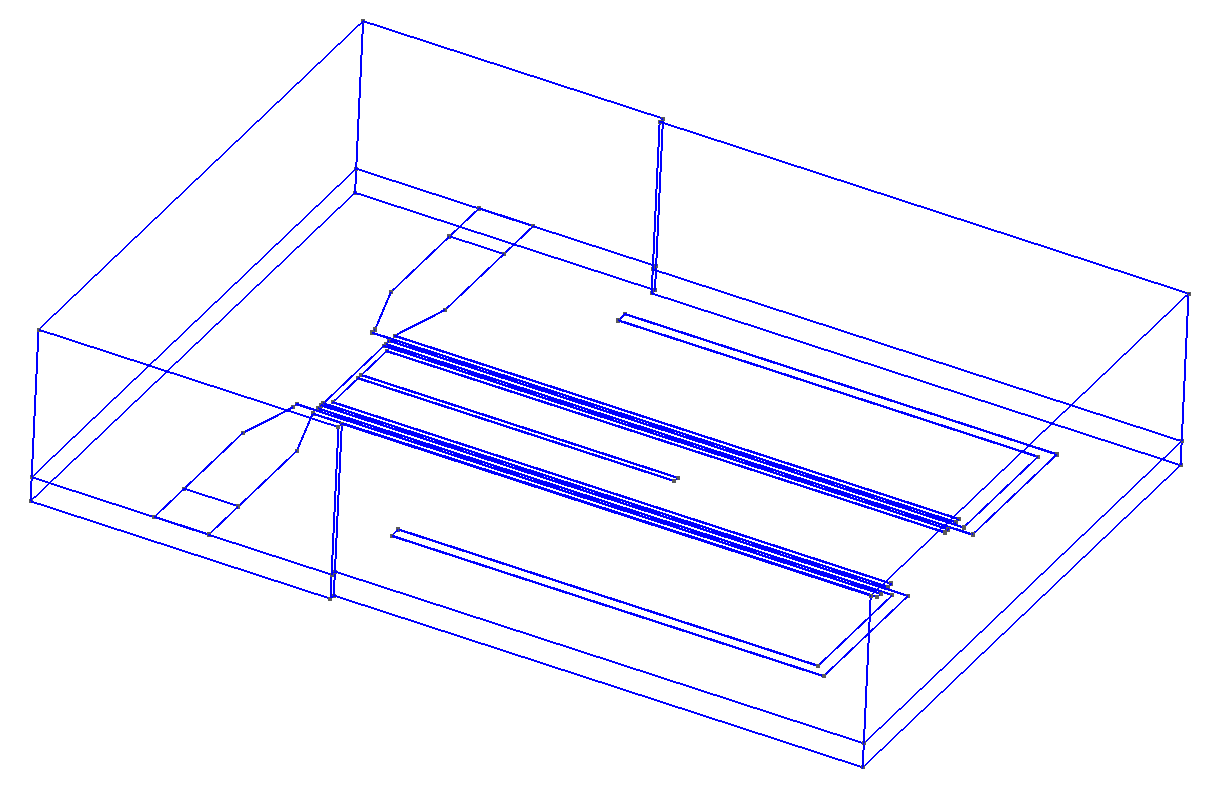
\includegraphics[width=0.7\textwidth]{../regression/OpenParEM3D/microstrip/filter_study/screenshots/filter_drawing}
  \caption{Microstrip filter drawing in FreeCAD.}
  \label{fig:filter_drawing}
\end{figure}
\begin{figure}[H]
  \centering
  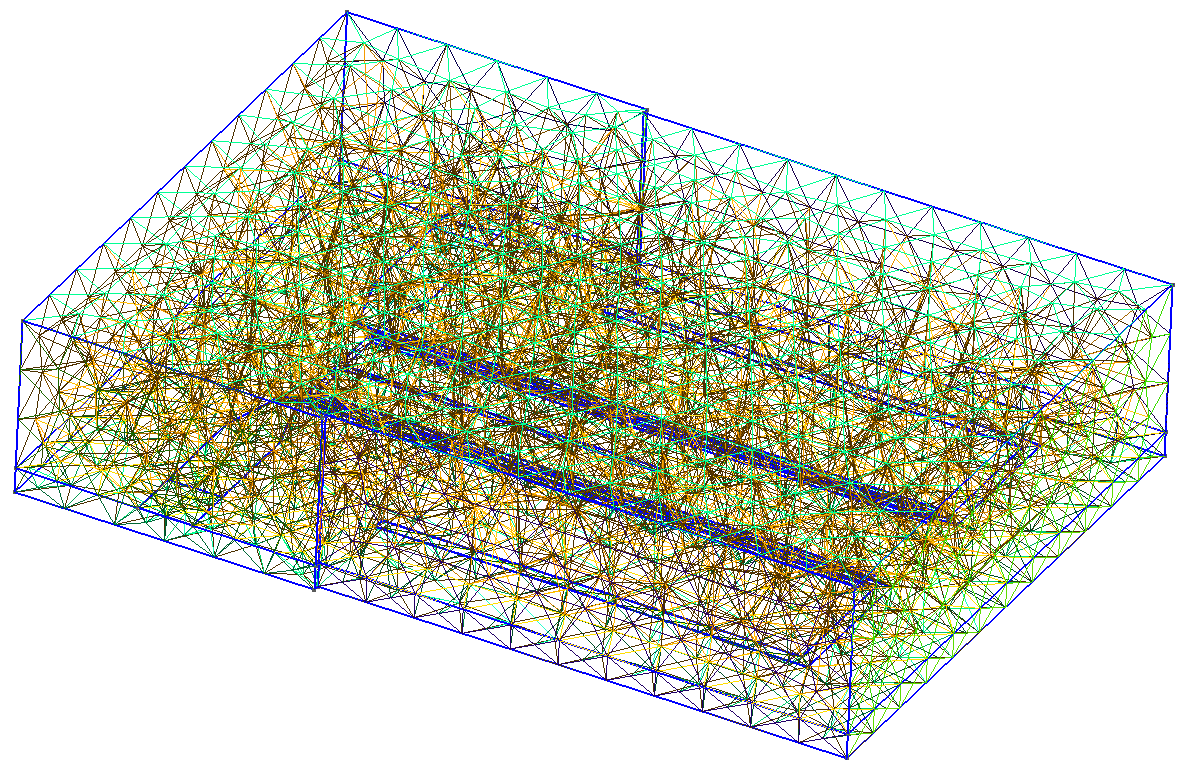
\includegraphics[width=0.7\textwidth]{../regression/OpenParEM3D/microstrip/filter_study/screenshots/filter_starting_mesh}
  \caption{Coarse starting mesh before adaptive refinement.}
  \label{fig:filter_starting_mesh}
\end{figure}

The simulation uses finite elements of order 1 through 5 with adaptive mesh refinement at 3~GHz using SandH refinement with reltol=0.02 and abstol of 2e-06 except for order~5, which does not use adaptive mesh refinement.  AMR is performed at 3~GHz to avoid very slow convergence for the initial 2D simulation at 0.5~GHz after AMR completes.  Simulation results are compared to the measurements in \cite{Weng} in Fig.~\ref{fig:filter_results} and Fig.~\ref{fig:filter_results_zoom}, and the agreement is quite good. 
\begin{figure}[p]
  \centering
  \begin{subfigure}{0.45\textwidth}
     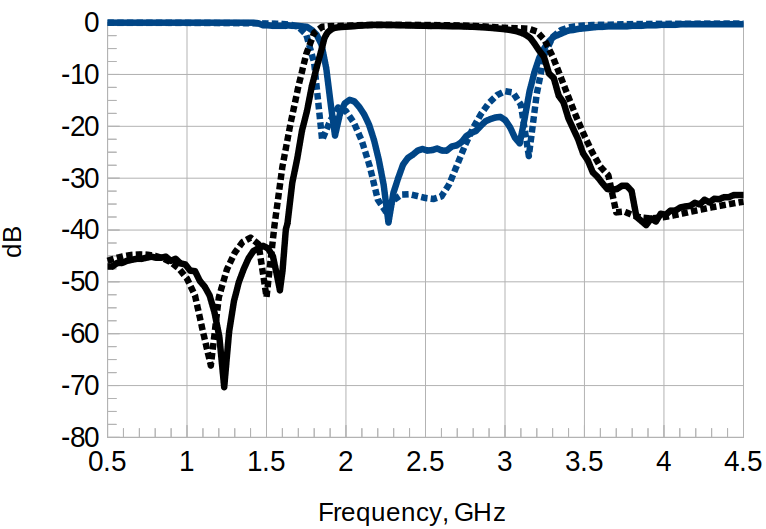
\includegraphics[width=\linewidth]{../regression/OpenParEM3D/microstrip/filter_study/screenshots/microstrip_filter_1st_order.png}
     \caption{1$^{\textnormal{st}}$ order.}
  \end{subfigure}
  \begin{subfigure}{0.45\textwidth}
     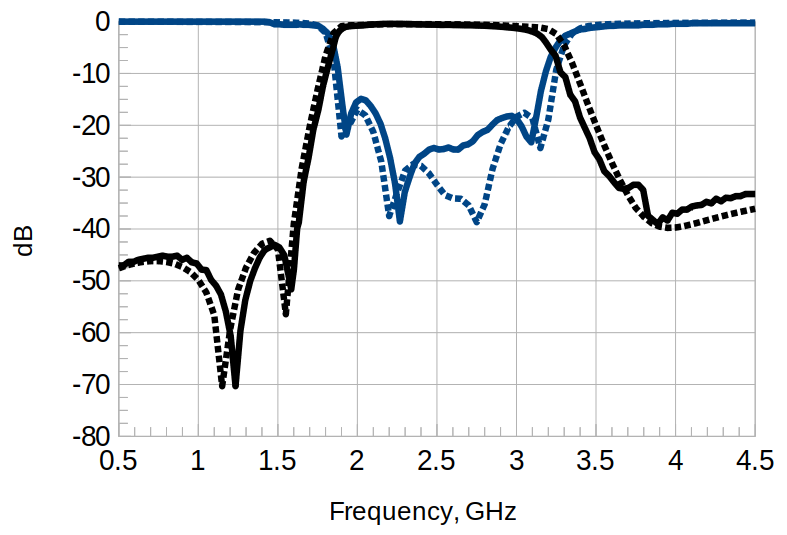
\includegraphics[width=\linewidth]{../regression/OpenParEM3D/microstrip/filter_study/screenshots/microstrip_filter_2nd_order.png}
     \caption{2$^{\textnormal{nd}}$ order.}
  \end{subfigure}
  \par\bigskip
  \begin{subfigure}{0.45\textwidth}
     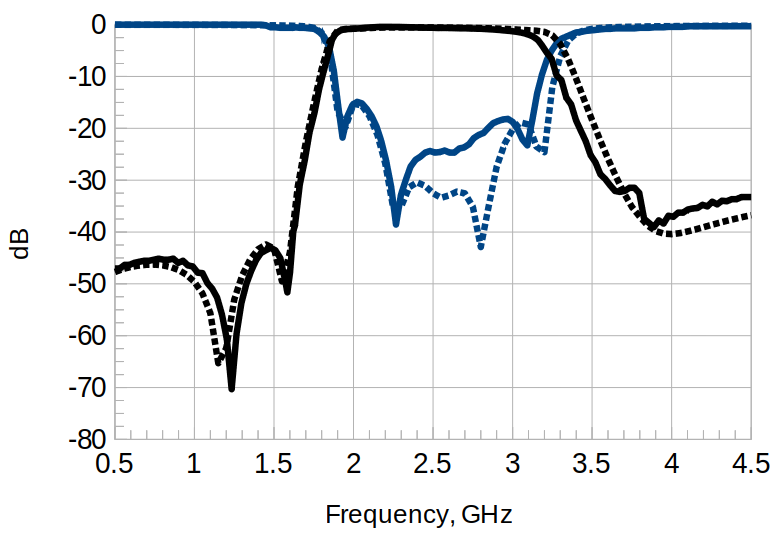
\includegraphics[width=\linewidth]{../regression/OpenParEM3D/microstrip/filter_study/screenshots/microstrip_filter_3rd_order.png}
     \caption{3$^{\textnormal{rd}}$ order.}
  \end{subfigure}
  \begin{subfigure}{0.45\textwidth}
     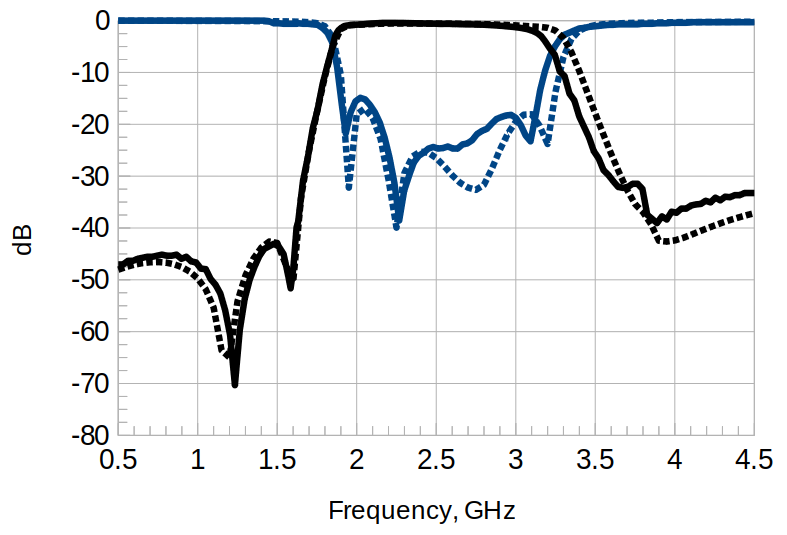
\includegraphics[width=\linewidth]{../regression/OpenParEM3D/microstrip/filter_study/screenshots/microstrip_filter_4th_order.png}
     \caption{4$^{\textnormal{th}}$ order.}
  \end{subfigure}
  \par\bigskip
  \begin{subfigure}{0.72\textwidth}
     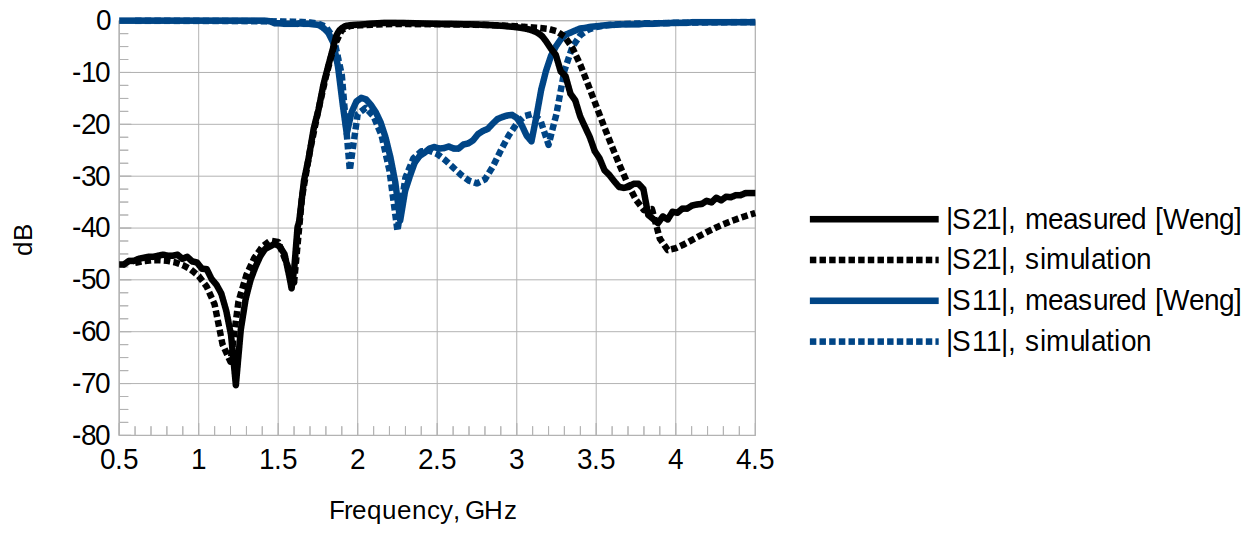
\includegraphics[width=\linewidth]{../regression/OpenParEM3D/microstrip/filter_study/screenshots/microstrip_filter_5th_order.png}
     \caption{5$^{\textnormal{th}}$ order.}
  \end{subfigure}
  \caption{S-parameter simulation results and comparison to experiment from \cite{Weng}.}
  \label{fig:filter_results}
\end{figure}
\begin{figure}[p]
  \centering
  \begin{subfigure}{0.45\textwidth}
     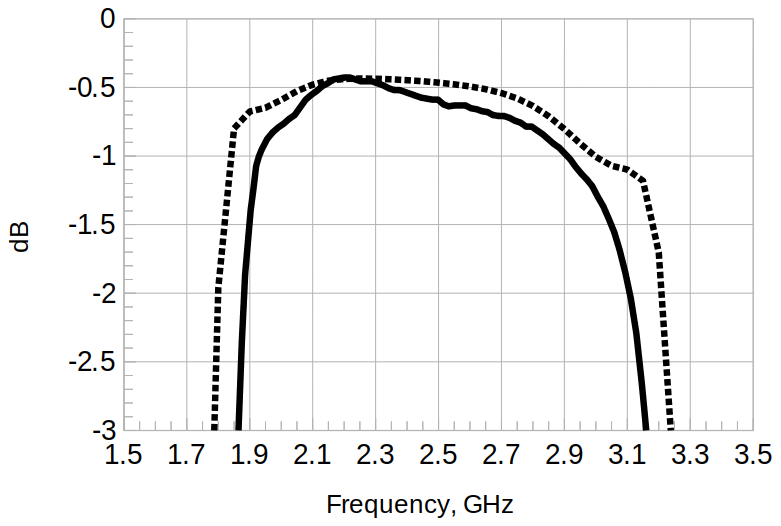
\includegraphics[width=\linewidth]{../regression/OpenParEM3D/microstrip/filter_study/screenshots/microstrip_filter_1st_order_zoom.png}
     \caption{1$^{\textnormal{st}}$ order.}
  \end{subfigure}
  \begin{subfigure}{0.45\textwidth}
     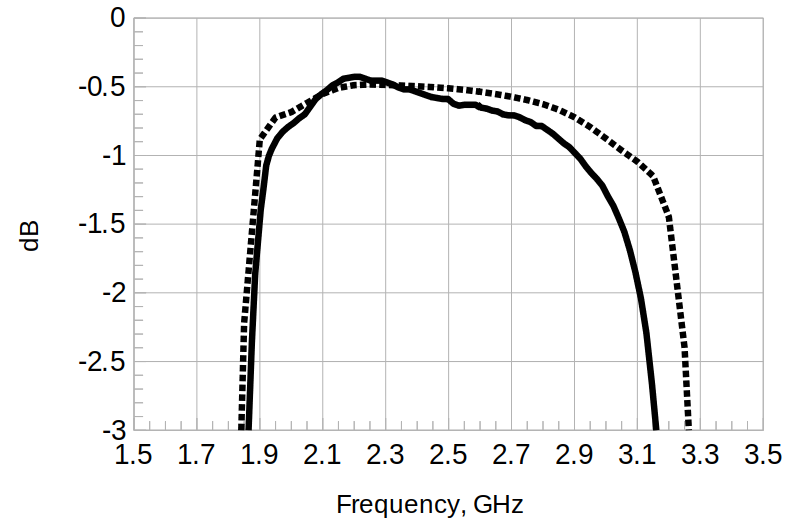
\includegraphics[width=\linewidth]{../regression/OpenParEM3D/microstrip/filter_study/screenshots/microstrip_filter_2nd_order_zoom.png}
     \caption{2$^{\textnormal{nd}}$ order.}
  \end{subfigure}
  \begin{subfigure}{0.45\textwidth}
     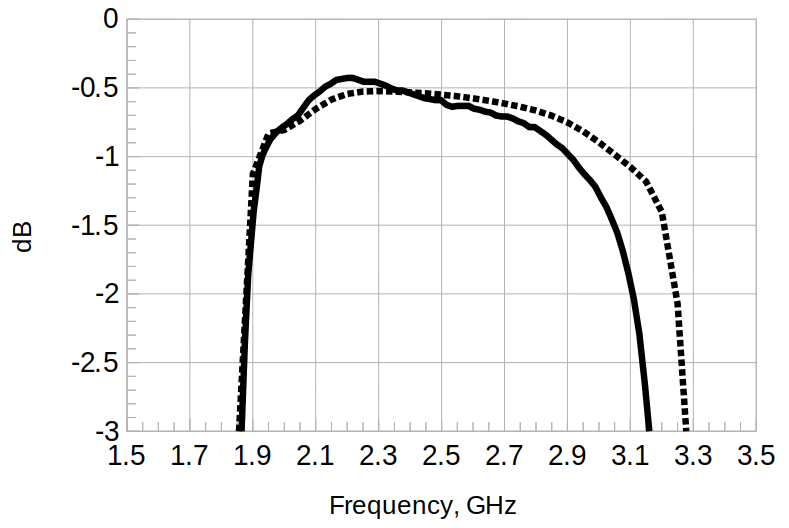
\includegraphics[width=\linewidth]{../regression/OpenParEM3D/microstrip/filter_study/screenshots/microstrip_filter_3rd_order_zoom.png}
     \caption{3$^{\textnormal{rd}}$ order.}
  \end{subfigure}
  \begin{subfigure}{0.45\textwidth}
     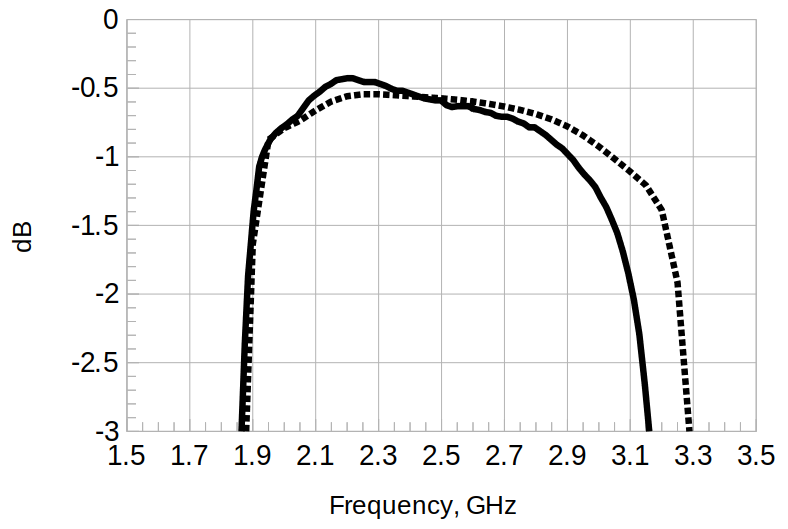
\includegraphics[width=\linewidth]{../regression/OpenParEM3D/microstrip/filter_study/screenshots/microstrip_filter_4th_order_zoom.png}
     \caption{4$^{\textnormal{th}}$ order.}
  \end{subfigure}
  \par\bigskip
  \begin{subfigure}{0.72\textwidth}
     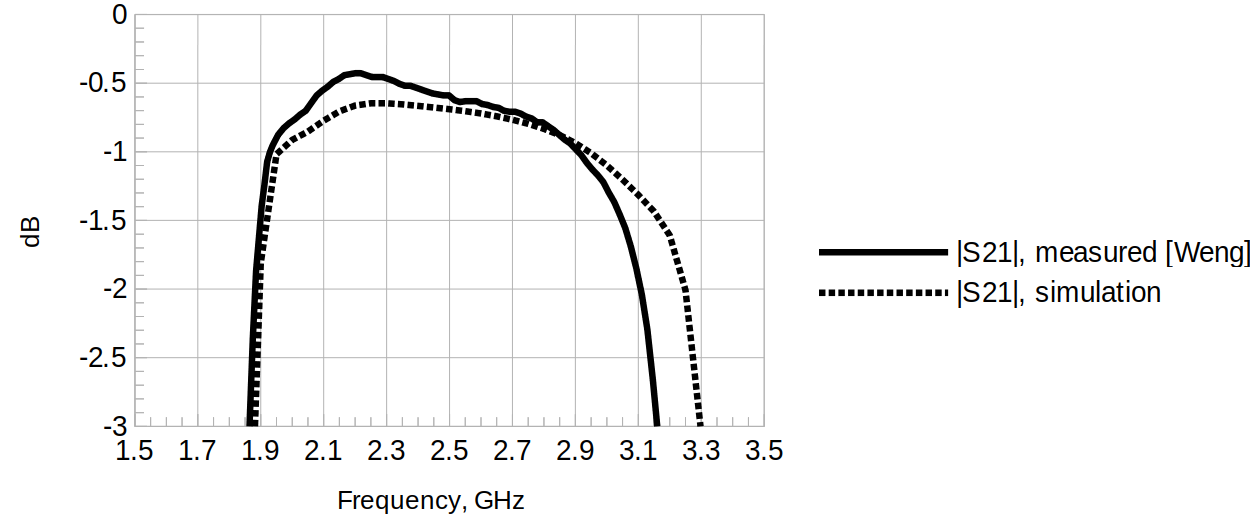
\includegraphics[width=\linewidth]{../regression/OpenParEM3D/microstrip/filter_study/screenshots/microstrip_filter_5th_order_zoom.png}
     \caption{5$^{\textnormal{th}}$ order.}
  \end{subfigure}
  \caption{Zoom of S-parameter simulation results and comparison to experiment from \cite{Weng}.}
  \label{fig:filter_results_zoom}
\end{figure}

Comparisons of the bandwidth and center frequencies are shown in Table~\ref{table:microstrip_filter_comparisons}, where agreement between measurement and simulation is good for all orders.  All five simulations produce slightly higher bandwidths, while increasing order shifts the center frequency higher.  Since the simulations use as-drawn values for dimensions and datasheet values for materials, it is not knowable which simulation is more accurate since they all fall within the manufacturing tolerances of the measured sample.
\begin{table}
\caption{Simulation vs. measurement comparisons.}
\begin{center}
\begin{tabular}{|c|c|c|}
\hline
Case & 3 dB BW, GHz & $f_c$, GHz \\
\hline
Measured \cite{Weng} & 1.26 & 2.51 \\
1$^{\textnormal{st}}$-order & 1.45 & 2.51 \\
2$^{\textnormal{nd}}$-order & 1.42 & 2.55 \\
3$^{\textnormal{rd}}$-order & 1.42 & 2.57 \\
4$^{\textnormal{rd}}$-order & 1.41 & 2.58 \\
5$^{\textnormal{rd}}$-order & 1.42 & 2.59 \\
\hline
\end{tabular}
\end{center}
\label{table:microstrip_filter_comparisons}
\end{table}

For 3$^{\textnormal{rd}}$-order elements, a slice of the refined mesh at the interface between the substrate and air including the bottom side of the conductor is shown in Fig.~\ref{fig:filter_refined_mesh}, where adaptive mesh refinement has added mesh elements to better resolve the traces.  For 3$^{\textnormal{rd}}$-order using this refined mesh and 5$^{\textnormal{th}}$-order elements using the un-refined starting mesh, the real part of magnitude of the magnetic field at 3~GHz is shown in Fig.~\ref{fig:filter_Hfield}.  Note that the scales are the same for the two plots.  A more refined plot can be obtained by tightening the convergence criteria and/or increasing the finite element order, but the run time would be greatly increased without a significant change to the S-parameters.
\begin{figure}[H]
  \centering
  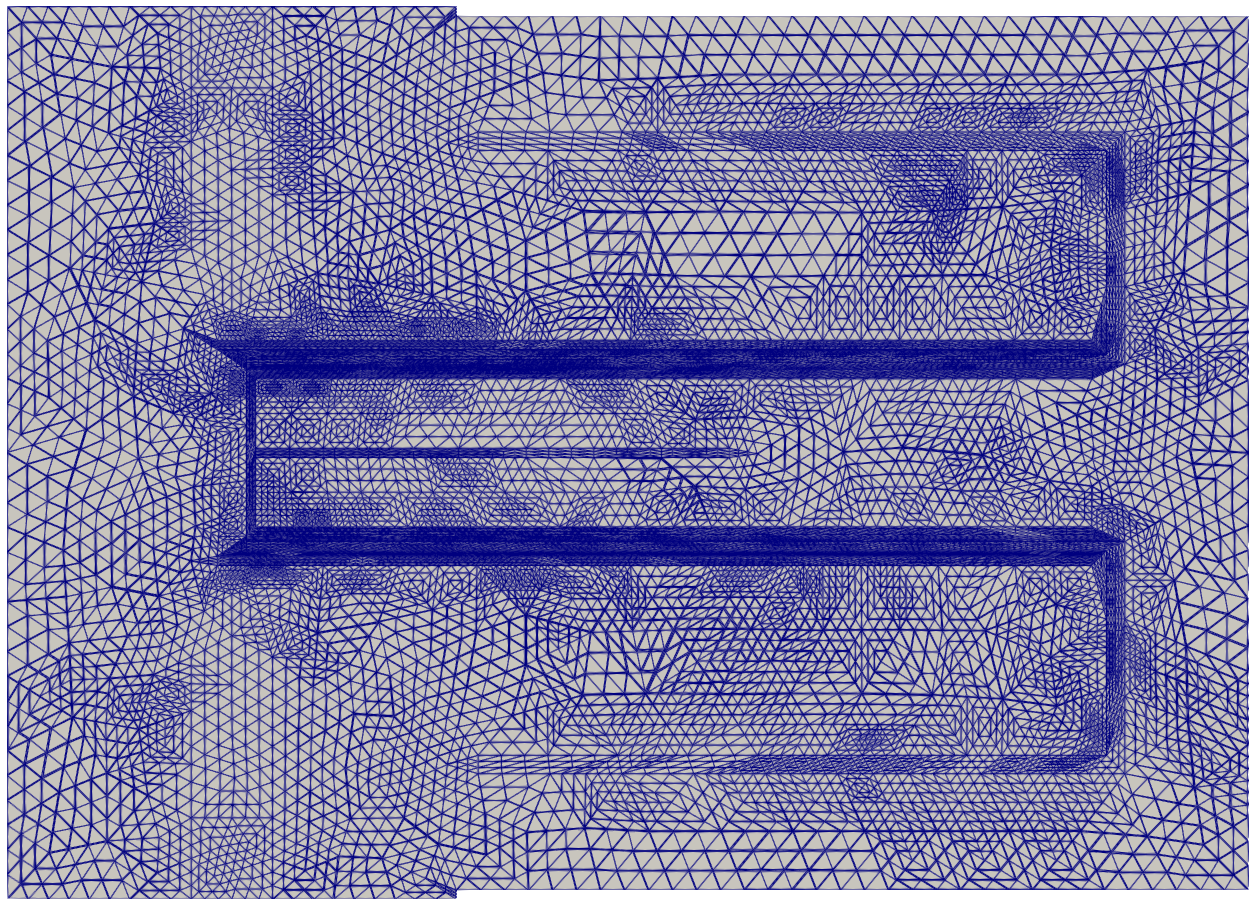
\includegraphics[width=0.55\textwidth]{../regression/OpenParEM3D/microstrip/filter_study/screenshots/filter_refined_mesh}
  \caption{Refined mesh for 3$^{\textnormal{rd}}$-order elements at the substrate/air interface including the bottom side of the metal traces.}
  \label{fig:filter_refined_mesh}
\end{figure}
\begin{figure}[H]
  \centering
  \begin{subfigure}{0.45\textwidth}
     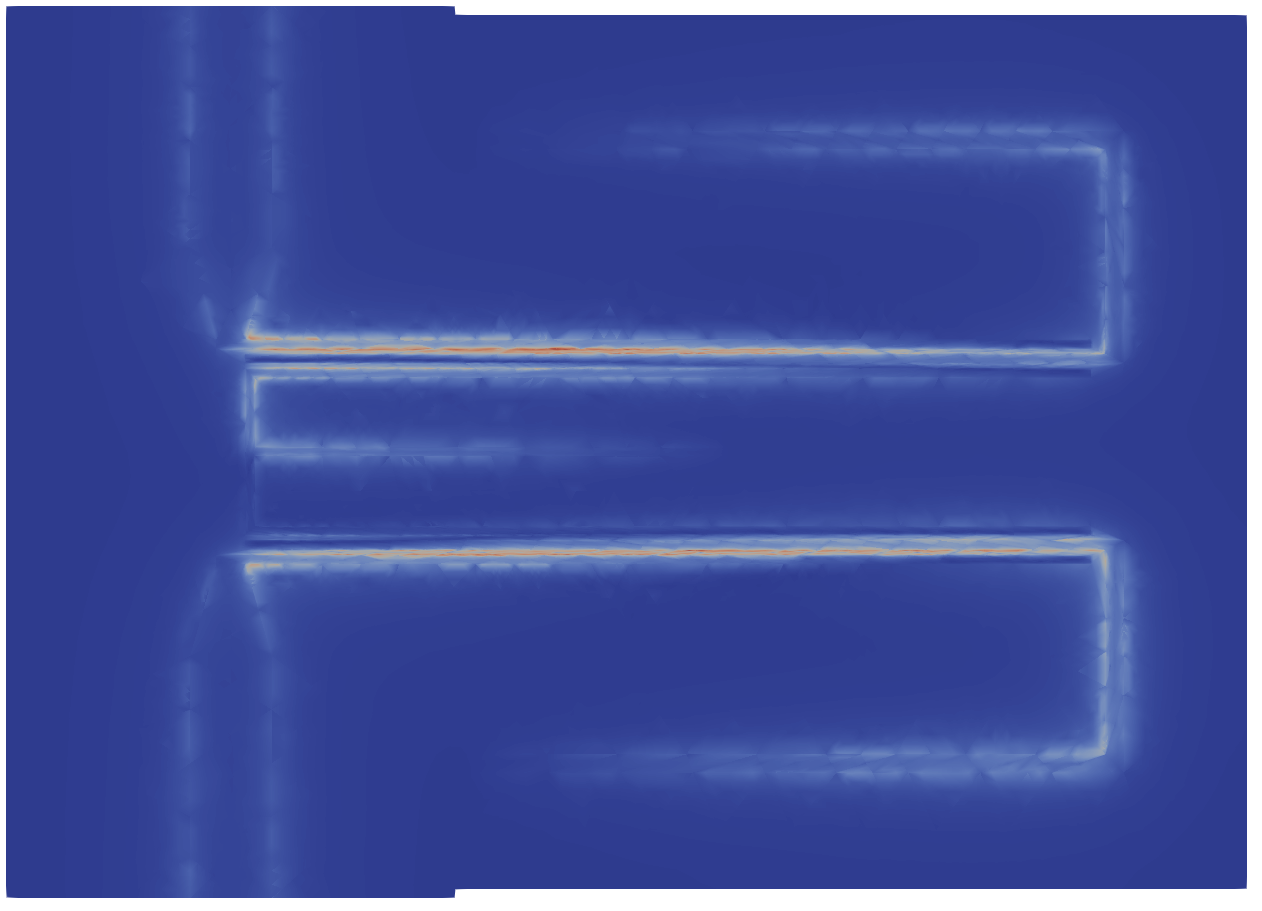
\includegraphics[width=\linewidth]{../regression/OpenParEM3D/microstrip/filter_study/screenshots/filter_3rd_order_Hfield}
     \caption{3$^{\textnormal{rd}}$ order \textit{with} adaptive refinement.}
  \end{subfigure}
  \begin{subfigure}{0.45\textwidth}
     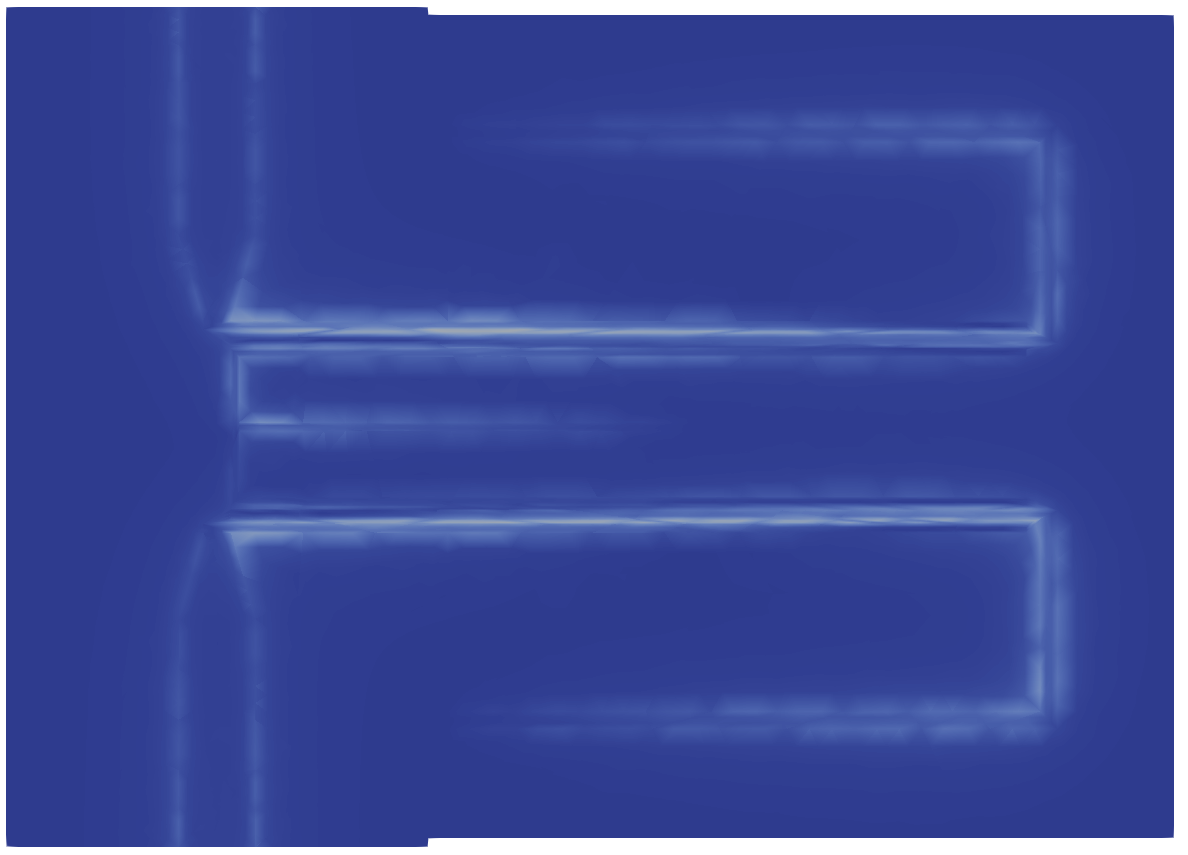
\includegraphics[width=\linewidth]{../regression/OpenParEM3D/microstrip/filter_study/screenshots/filter_5th_order_Hfield}
     \caption{5$^{\textnormal{th}}$ order \textit{without} adaptive refinement.}
  \end{subfigure}
  \caption{Plots of Re$(|\overline{H}|)$ at the substrate/air interface including the bottom side of the metal traces.}
  \label{fig:filter_Hfield}
\end{figure}

Various counts and run times are shown in Fig.~\ref{fig:filter_run_times}. In (a), lower finite element orders require more iterations to achieve convergence, leading to larger meshes at lower orders, as shown in (b) with the solid line.  However, lower-order elements require fewer degrees of freedom (DOF) per element, and the dashed line in (b) shows that the DOF count is more similar across the various orders, but higher-order elements still trend to requiring lower DOF counts.  The net result on run time is shown in (c) with the solid line, where run times decrease with higher orders before increasing again, producing a minimum for best run time.  The order that produces the shortest run time is dependent on the computer.  

The starting mesh for the ports have very high aspect ratio elements ($\approx 102$) that cause convergence difficulties for higher-order finite elements during the initial solve, after which, the previous solution is used as the initial guess, and no further issues are encountered.  The dashed line in Fig.~\ref{fig:filter_run_times}(c) shows the run times with excess 2D solve time for the initial solve removed.  The effect becomes more noticeable for higher orders, indicating a potential benefit of providing support for an initial guess at the first 2D solve.

\begin{figure}[H]
  \centering
  \begin{subfigure}[t]{0.38\textwidth}
     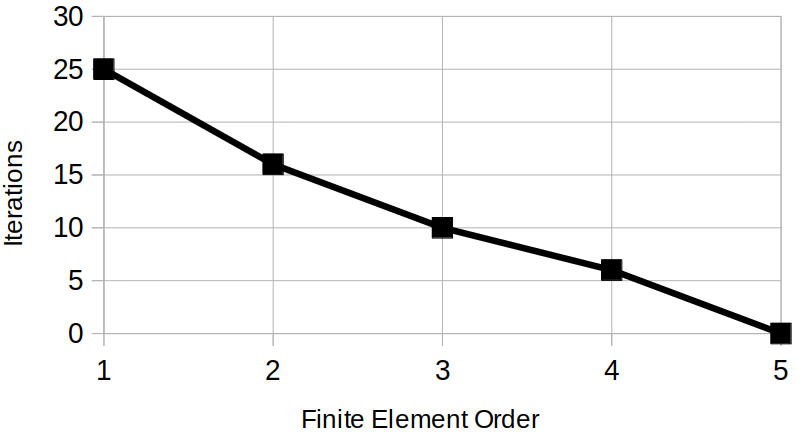
\includegraphics[width=1\linewidth]{../regression/OpenParEM3D/microstrip/filter_study/screenshots/filter_iterations}
     \caption{Iteration counts.}
  \end{subfigure}
  \begin{subfigure}[t]{0.43\textwidth}
     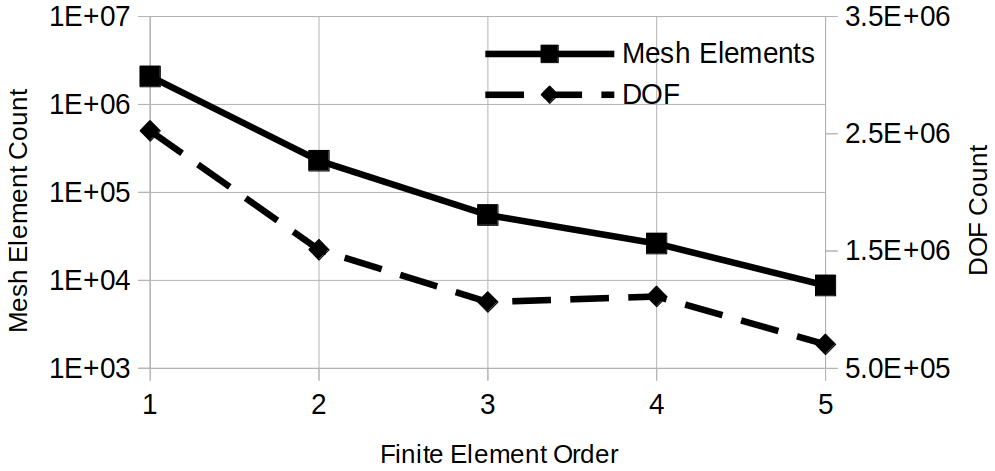
\includegraphics[width=1\linewidth]{../regression/OpenParEM3D/microstrip/filter_study/screenshots/filter_counts}
     \caption{Mesh and DOF counts.}
  \end{subfigure}
  \par\bigskip
  \begin{subfigure}[t]{0.35\textwidth}
     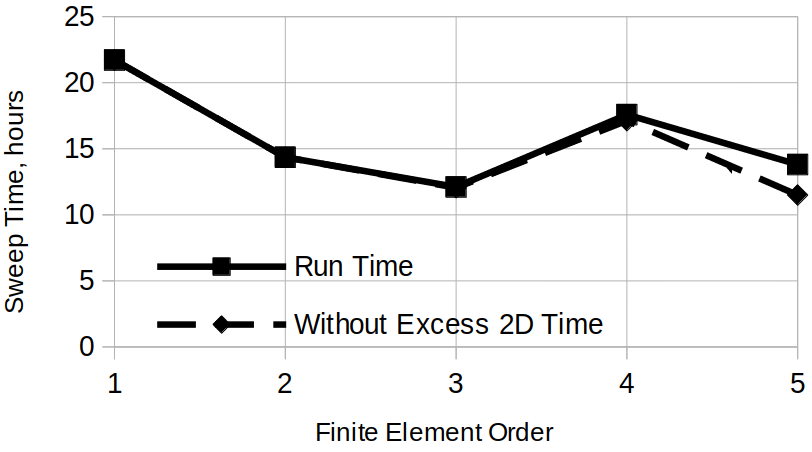
\includegraphics[width=1\linewidth]{../regression/OpenParEM3D/microstrip/filter_study/screenshots/filter_run_times}
     \caption{Run times.}
  \end{subfigure}
  \caption{Performance metrics vs. finite element order.}
  \label{fig:filter_run_times}
\end{figure}

\subsection{Square Monopole Antenna}

The planar monopole antenna described in \cite{Wong} is simulated for comparison with the paper's measurement.  The project can be found in the OpenParEM distribution in \texttt{regression/OpenParEM3D/antenna/square\_monopole\_study}.  The layout is done in FreeCAD following the dimensions from the paper, and the final drawing is shown in Fig.~\ref{fig:square_planar_drawing} along with the coaxial feed with the port outlined in green.  The paper does not describe how the antenna mounts to the connector, how the connector pin is treated, nor the drilled hole size in the ground plane, so the drawn antenna makes reasonable guesses at these, but some impact on the results is expected.

\begin{figure}[H]
  \centering
  \begin{subfigure}[t]{0.38\textwidth}
     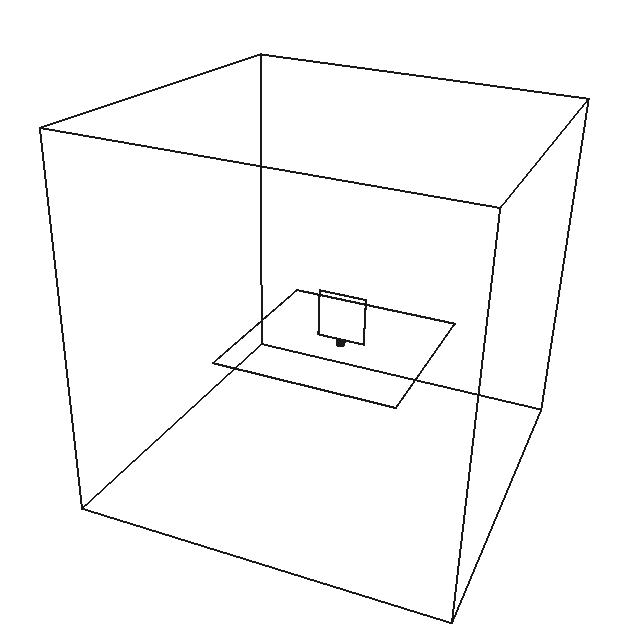
\includegraphics[width=0.95\linewidth]{../regression/OpenParEM3D/antenna/square_monopole_study/screenshots/drawing}
     \caption{Square planar monopole drawing in FreeCAD.}
  \end{subfigure}
  \begin{subfigure}[t]{0.38\textwidth}
     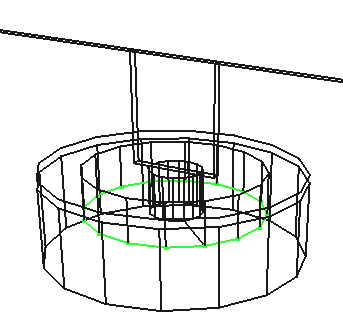
\includegraphics[width=0.95\linewidth]{../regression/OpenParEM3D/antenna/square_monopole_study/screenshots/drawing_zoom}
     \caption{Zoom of coaxial feed with the port outlined in green.}
  \end{subfigure}
  \caption{Square planar monopole drawing in FreeCAD.}
  \label{fig:square_planar_drawing}
\end{figure}

For an antenna, the mesh must be sufficiently fine in the entire domain to accurately represent the radiating fields.  Use of higher-order finite elements allows the mesh density to be pre-set to accurately simulate the radiating far fields.  Since electromagnetic fields in the far field take a sinusoidal distribution, the maximum element size can be determined by how well an N$^{\textnormal{th}}$-order polygon fits a sinusoid.  A 3$^{\textnormal{rd}}$-order element can fit a half-wavelength sinusoid to about 0.8\% accuracy, which is sufficient for this work.  The free-space wavelength at 6~GHz is 50~mm for a half-wavelength of 25~mm.  The mesh is generated by gmsh using default settings except that the maximum element size is limited to 25~mm.

The simulation uses finite elements of order 3 with adaptive mesh refinement at 12~GHz using S refinement with reltol=0.01.  The material for the metals is defaulted to brass, and radiation boundary conditions are applied to the outer cube surface.  Simulation results are compared to the measurements in \cite{Wong} in Fig.~\ref{fig:square_monopole_results}, and the agreement is good considering the uncertainty of the physical construction at the antenna mounting location.
\begin{figure}[H]
  \centering
  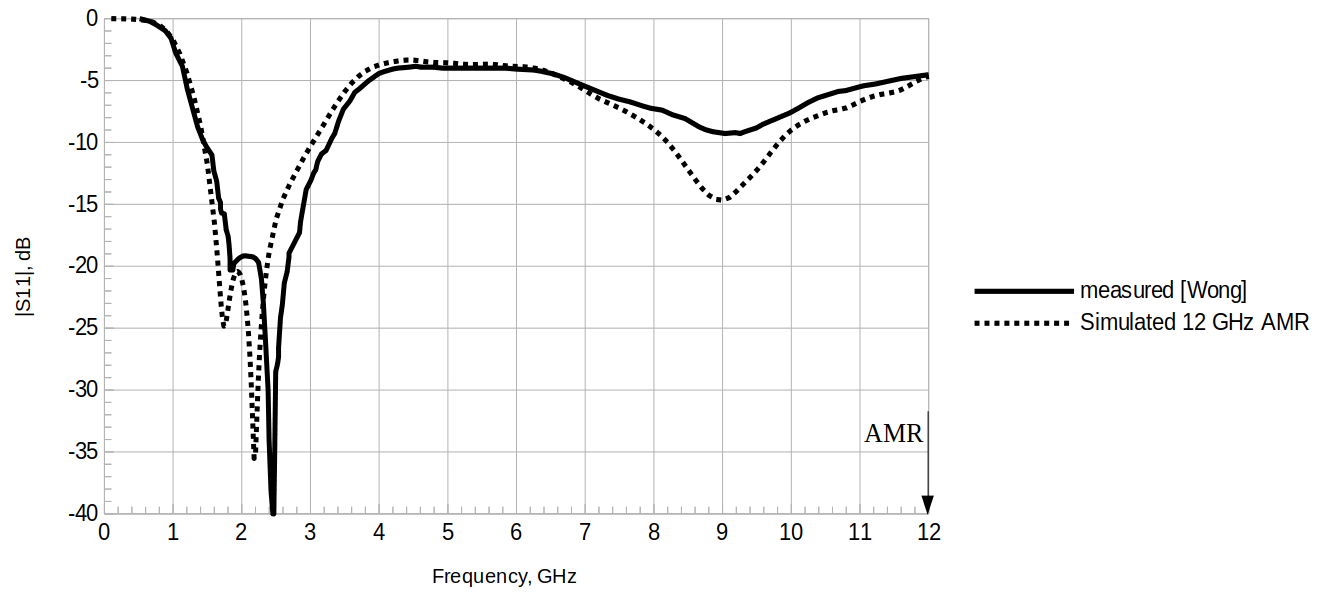
\includegraphics[width=0.75\textwidth]{../regression/OpenParEM3D/antenna/square_monopole_study/screenshots/results_12GHz_AMR}
  \caption{S-parameter simulation results with AMR at 12 GHz and comparison to experiment from \cite{Wong}.}
  \label{fig:square_monopole_results}
\end{figure}

A second simulation is performed with adaptive mesh refinement at 3~GHz instead of 12~GHz.  At 3~GHz, adaptive mesh refinement is only needed in quasi-static areas with sharp field changes since the sinusoidal areas are automatically accommodated by the 3$^{\textnormal{rd}}$-order finite elements combined with the maximum mesh element size of 25~mm.  Simulation results are compared to the measurements in \cite{Wong} in Fig.~\ref{fig:square_monopole_results_3GHz}, and the results look practically identical up to 8~GHz compared to those in Fig.~\ref{fig:square_monopole_results} using AMR at 12~GHz.  So the adaptive mesh refinement addresses the sharp quasi-static field changes while the 3$^{\textnormal{rd}}$-order elements and maximum mesh element size addresses the radiating field resulting in a solution good to 6~GHz at about 0.8\% sinusoidal fitting accuracy.  The plot shows visible differences above 8~GHz because the 3$^{\textnormal{rd}}$-order polynomial fitting error climbs to 4\% at 8~GHz (2/3 wavelength) with the fitting error increasing with frequency.
\begin{figure}[H]
  \centering
  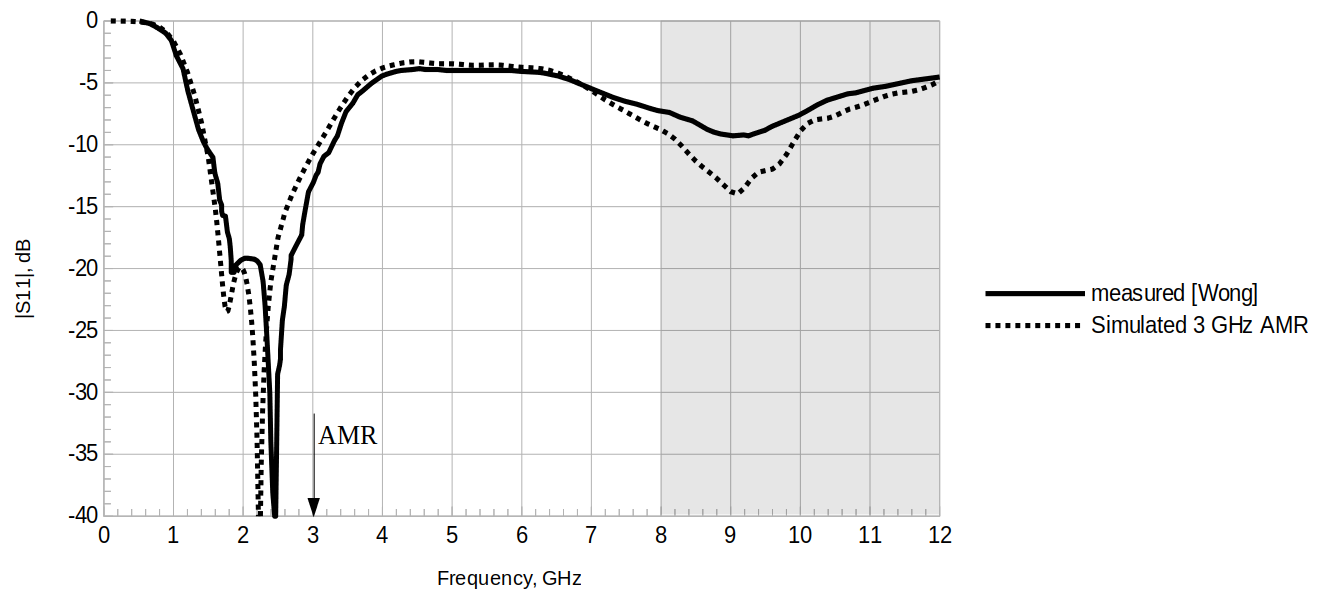
\includegraphics[width=0.75\textwidth]{../regression/OpenParEM3D/antenna/square_monopole_study/screenshots/results_3GHz_AMR}
  \caption{S-parameter simulation results with AMR at 3 GHz and comparison to experiment from \cite{Wong}.}
  \label{fig:square_monopole_results_3GHz}
\end{figure}

To summarize, higher-order finite elements enable a strategy for antennas of avoiding adaptive mesh refinement in the near-to-far-field region by setting the maximum mesh element size based on the highest frequency of interest and the finite element order.  AMR then focuses on the quasi-static regions with sharp field changes.  In a sense, this results in an optimal simulation strategy by using AMR where it is needed and avoiding it where it is not.  A few fitting errors are shown in Table~\ref{table:fitting_errors}, where the expected pattern of increasing error with element size for a given finite element order and decreasing error with finite element order for a given element size is observed.

\begin{table}[H]
\caption{Errors for Wavelength vs. Polynomial Order for Fitting Sinusoids}
\begin{center}
\begin{tabular}{|c|c|c|}
\hline
Order & Wavelength Fraction & Fitting Error \\
\hline
2 & 0.25 & 0.0020 \\
2 & 0.5 & 0.028 \\
3 & 0.25 & 0.00028 \\
3 & 0.5 & 0.0081 \\
3 & 0.666 & 0.040 \\
3 & 1 & 0.18 \\
4 & 0.5 & 0.0010 \\
4 & 0.75 & 0.011 \\
\hline
\end{tabular}
\end{center}
\label{table:fitting_errors}
\end{table}
 

\subsection{Microstrip Bridge}

The microstrip bridge described in \cite{Wang} is simulated for comparison with the paper's simulation.  The bridge inserts a break in a microstrip line with the conductor bridging between the two microstrip sections through an area that is uniformly filled with a dielectric taking values of 1, 2.32, 3.78, and 9.8.  The project can be found in the OpenParEM distribution in \texttt{regression/OpenParEM3D/microstrip/bridge\_study}.  The layout is done in FreeCAD following the dimensions from the paper, and the final drawing is shown in Fig.~\ref{fig:bridge_drawing}.  Meshing uses gmsh with all default settings except that the mesh "Element size factor" is set to 0.5 to reduce the number of large elements.

\begin{figure}[H]
  \centering
  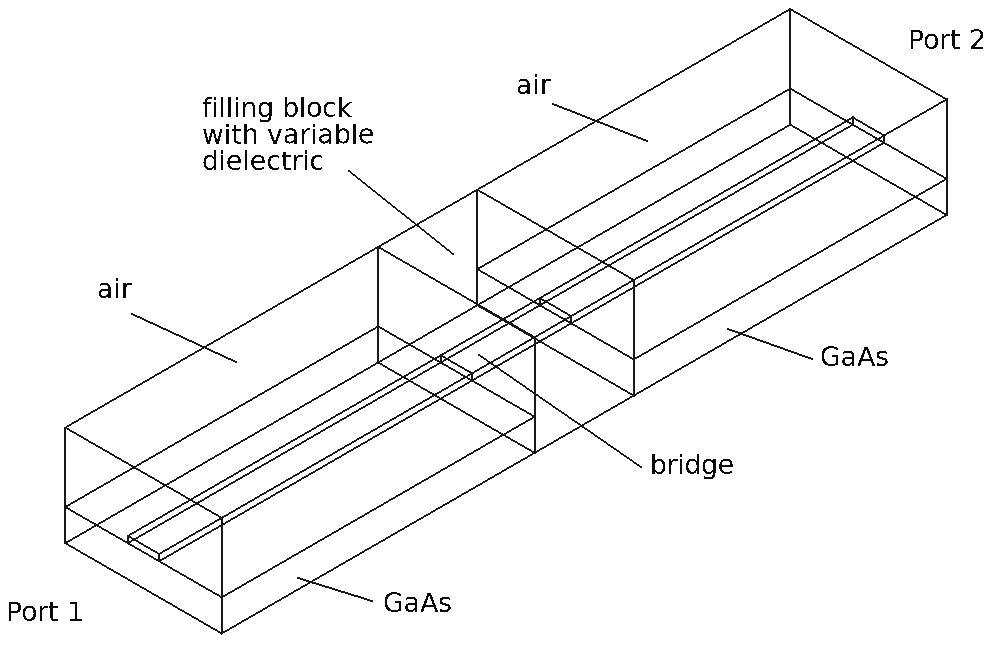
\includegraphics[width=0.5\textwidth]{../regression/OpenParEM3D/microstrip/bridge_study/screenshots/bridge_drawing}
  \caption{Drawing of a microstrip bridge across a gap with variable dielectric constant filling.}
  \label{fig:bridge_drawing}
\end{figure}

At the highest frequency in the simulation, the longest mesh element in any material is just 0.21$\lambda$, enabling 5$^{\textnormal{th}}$-order elements are to be used without adaptive mesh refinement.  The mesh used at all frequencies is shown in Fig.~\ref{fig:bridge_mesh}.

\begin{figure}[H]
  \centering
  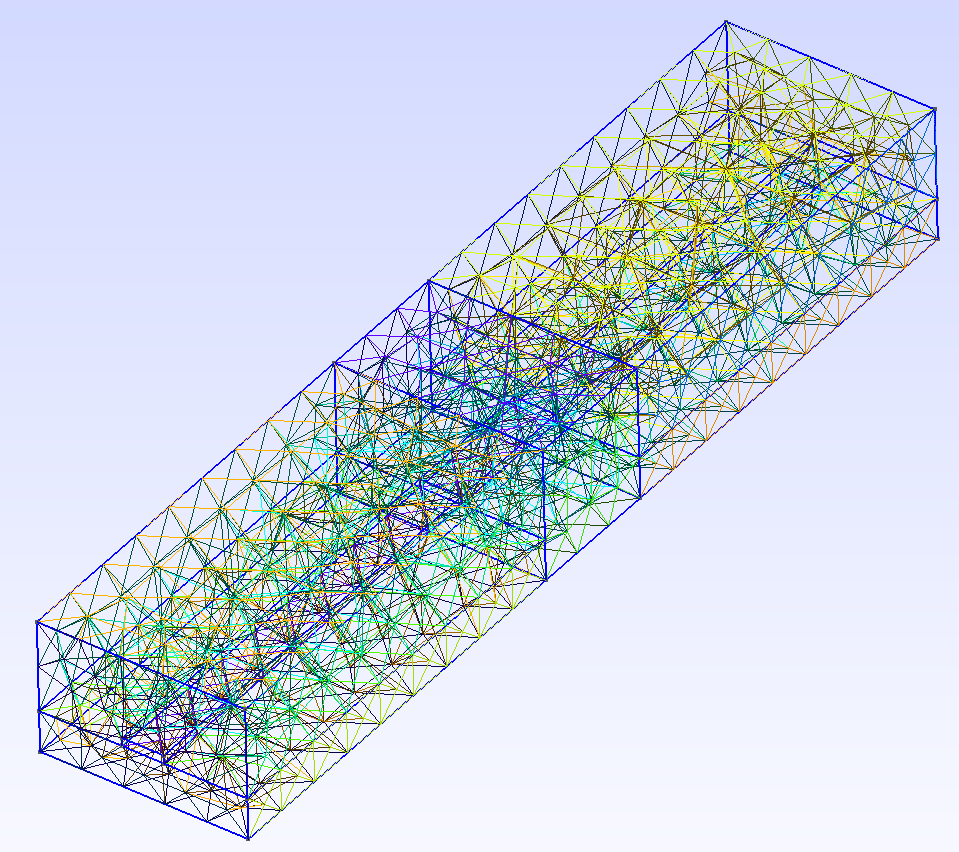
\includegraphics[width=0.5\textwidth]{../regression/OpenParEM3D/microstrip/bridge_study/screenshots/bridge_mesh}
  \caption{Mesh used for the analysis of the microstrip bridge.}
  \label{fig:bridge_mesh}
\end{figure}

Results are shown in Fig.~\ref{fig:bridge_results}, where the agreement with \cite{Wang} is excellent.  The results here do not show the small level of "waviness" with respect to frequency that reference \cite{Wang} show.  Given the short electrical length of the bridge and its simplicity, there is no physical mechanism to generate the waviness observed in the results of \cite{Wang}, so it is assumed that the waviness an artifact of the simulation in \cite{Wang}.

\begin{figure}[H]
  \centering
  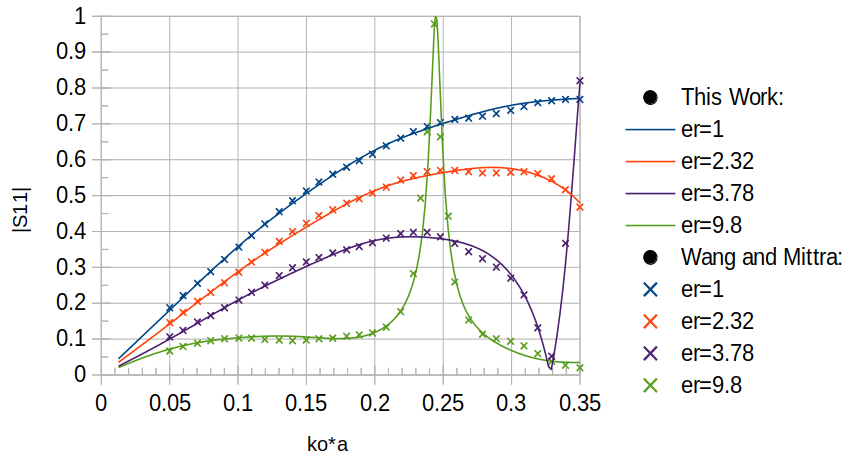
\includegraphics[width=0.75\textwidth]{../regression/OpenParEM3D/microstrip/bridge_study/screenshots/bridge_results}
  \caption{Simulation results with comparison to \cite{Wang} using 5$^{\textnormal{th}}$-order elements \textit{without} adaptive mesh refinement.}
  \label{fig:bridge_results}
\end{figure}

It is interesting to note that the simulation with  5$^{\textnormal{th}}$-order elements supports a $167\times$ range of frequency over a $9.8\times$ range of dielectric constant with the same mesh that has no adaptive mesh refinement.  The performance is even achieved for microstrip with finite-thickness metal and sharp edges with no special treatment of the mesh at the edges.

\subsection{Slotline Step}

The slotline step in width described in \cite{Hirayama} is simulated for comparison with the paper's simulation.  The project can be found in the OpenParEM distribution in \texttt{regression/OpenParEM3D/slotline/step\_study}.  Applying symmetry, half of the structure is drawn in FreeCAD following the dimensions from the paper, and the final drawing is shown in Fig.~\ref{fig:step_drawing}.  Meshing uses gmsh with all default settings.

\begin{figure}[H]
  \centering
  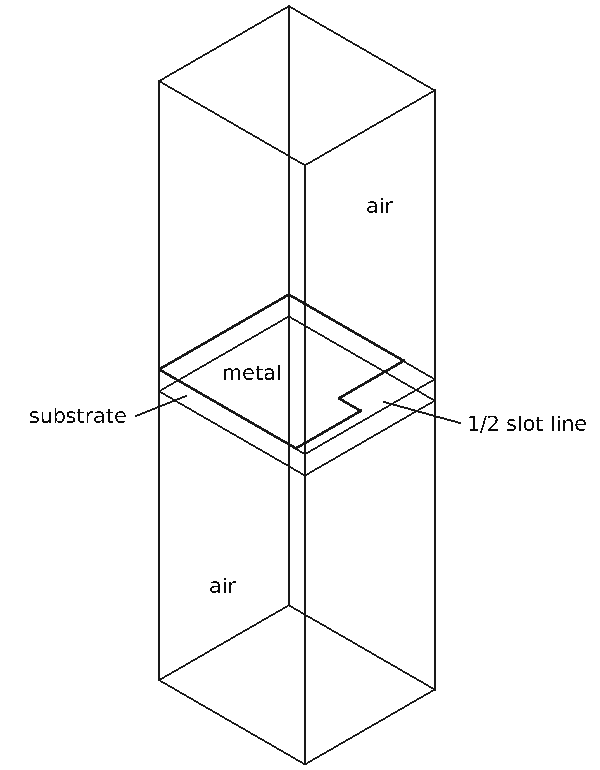
\includegraphics[width=0.45\textwidth]{../regression/OpenParEM3D/slotline/step_study/screenshots/step_drawing}
  \caption{Drawing of 1/2 of a slotline step in width.}
  \label{fig:step_drawing}
\end{figure}

The simulation uses 3$^{\textnormal{rd}}$-order elements and adaptive mesh refinement at 35~GHz with convergence on S using a relative tolerance of 0.001 with two consecutive iterations.  The results and comparison to those of \cite{Hirayama} are shown in Fig.~\ref{fig:step_results}, where the agreement is excellent.  A plot of $\textnormal{Re}(|\overline{H}|)$ on the substrate side of the metal and the slotline gap at 35~GHz when driving the step from the narrow end is shown in Fig.~\ref{fig:step_plot}.  Note the use of amplitude discretization to visualize equipotential lines.

\begin{figure}[H]
  \centering
  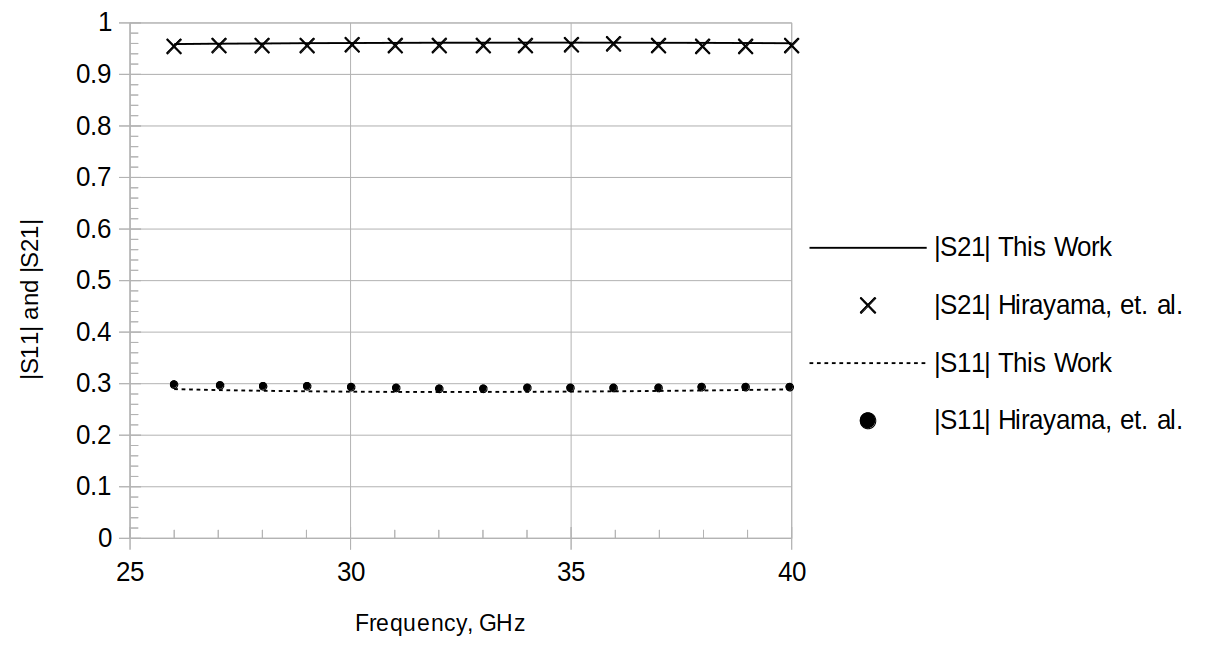
\includegraphics[width=0.8\textwidth]{../regression/OpenParEM3D/slotline/step_study/screenshots/step_results}
  \caption{Simulation results with comparison to \cite{Hirayama} using 3$^{\textnormal{rd}}$-order elements with adaptive mesh refinement.}
  \label{fig:step_results}
\end{figure}

\begin{figure}[H]
  \centering
  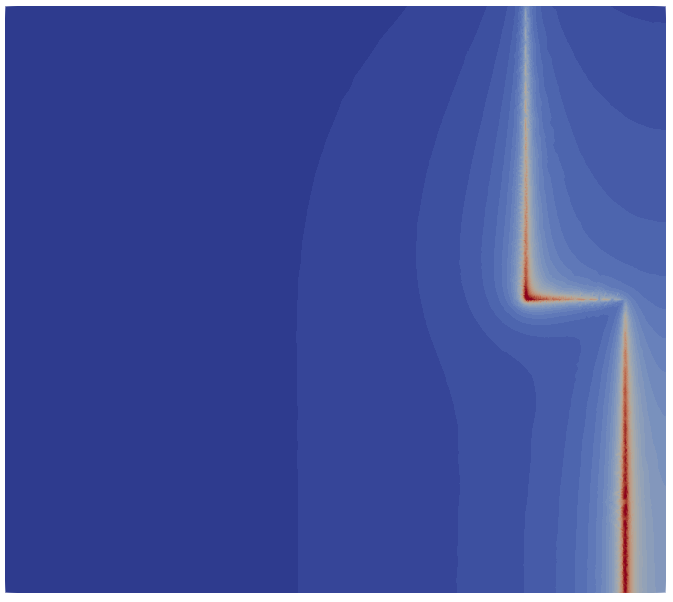
\includegraphics[width=0.7\textwidth]{../regression/OpenParEM3D/slotline/step_study/screenshots/step_real_H}
  \caption{Plot of $\textnormal{Re}(|\overline{H}|)$ at 35~GHz driving the narrow end.}
  \label{fig:step_plot}
\end{figure}

\subsection{Waveguide T-Junction}

The WR75 T-Junction described in \cite{Alessandri} is simulated for comparison with the paper's simulation.  The project is in the OpenParEM distribution in \texttt{regression/OpenParEM3D/WR75/T-Junction\_study}.  The structure is drawn in FreeCAD as shown in Fig.~\ref{fig:junction_drawing}.  Shown in Fig.~\ref{fig:junction_mesh}, the mesh is built using gmsh with all default settings except that the mesh "Element size factor" is set to 0.75.

\begin{figure}[H]
  \centering
  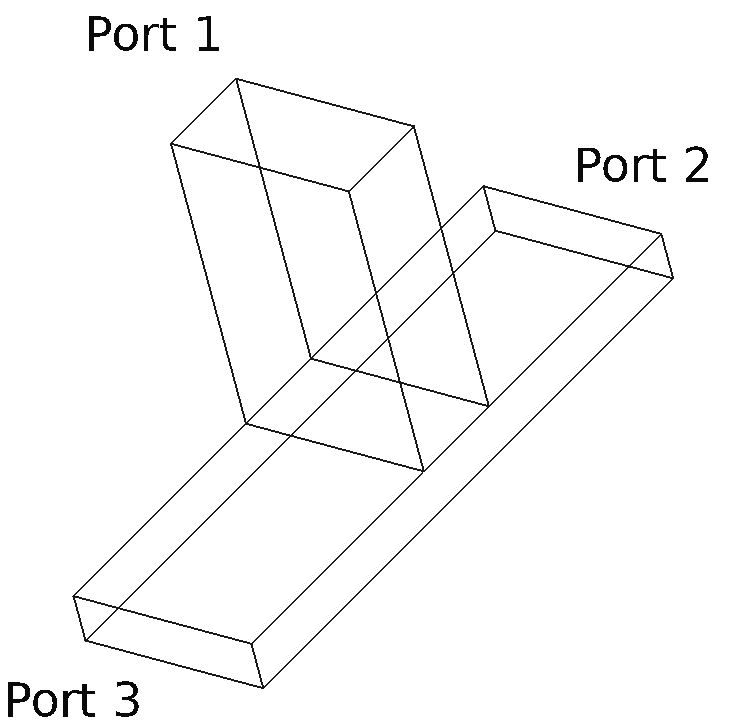
\includegraphics[width=0.4\textwidth]{../regression/OpenParEM3D/WR75/T-Junction_study/screenshots/junction_drawing}
  \caption{Drawing of a WR75 T-Junction.}
  \label{fig:junction_drawing}
\end{figure}

\begin{figure}[H]
  \centering
  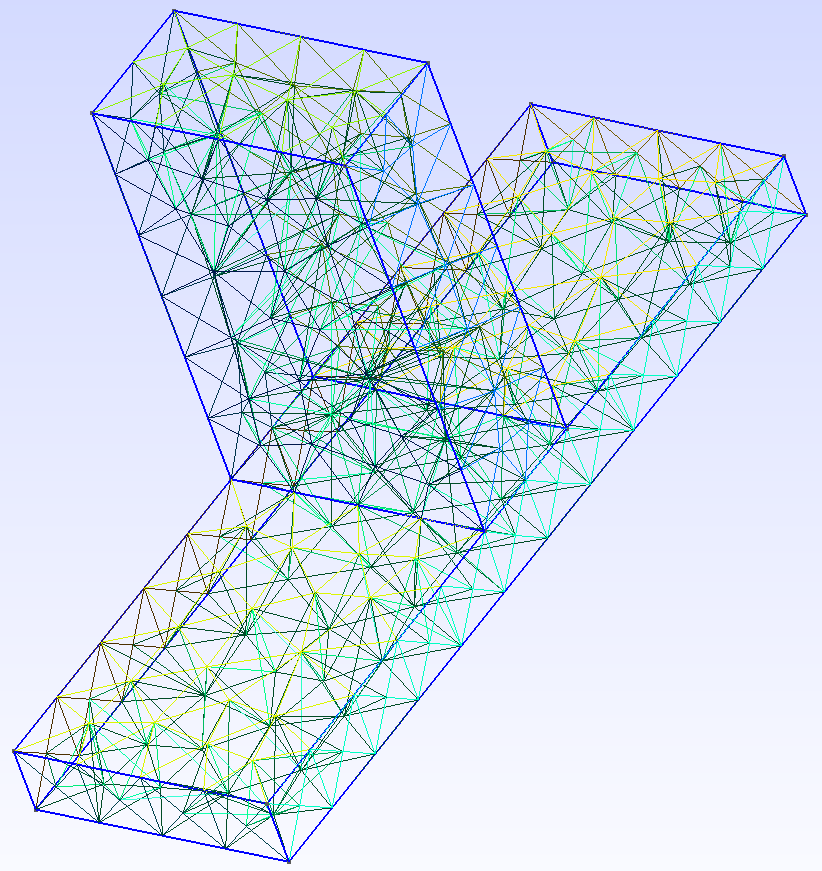
\includegraphics[width=0.25\textwidth]{../regression/OpenParEM3D/WR75/T-Junction_study/screenshots/junction_mesh}
  \caption{Mesh for the WR75 T-Junction.}
  \label{fig:junction_mesh}
\end{figure}

The simulation uses 4$^{\textnormal{th}}$-order elements with no adaptive refinement, and the results and comparisons to \cite{Alessandri} are shown in Fig.~\ref{fig:junction_results}. The agreement is excellent.

\begin{figure}[H]
  \centering
  \begin{subfigure}[t]{0.49\textwidth}
     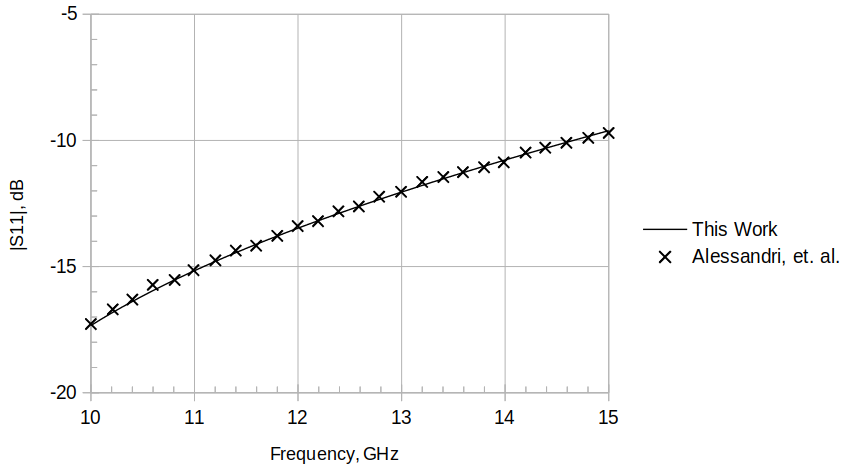
\includegraphics[width=0.95\linewidth]{../regression/OpenParEM3D/WR75/T-Junction_study/screenshots/junction_S11}
     \caption{S11.}
  \end{subfigure}
  \begin{subfigure}[t]{0.49\textwidth}
     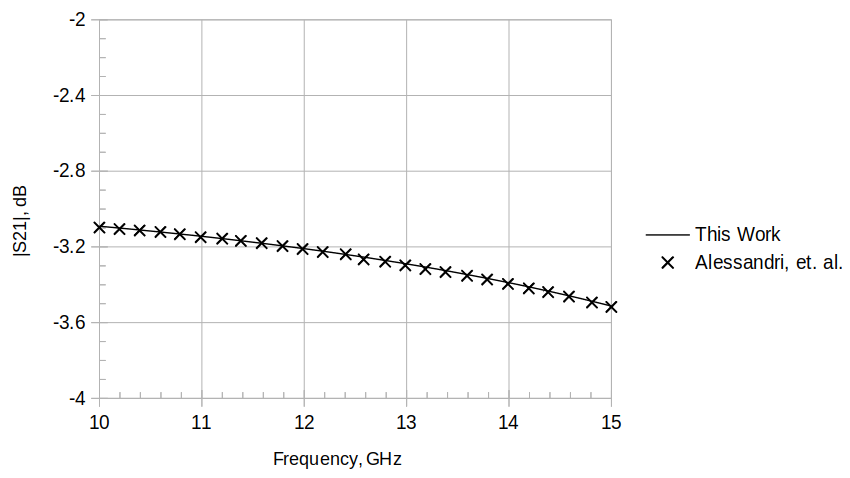
\includegraphics[width=0.95\linewidth]{../regression/OpenParEM3D/WR75/T-Junction_study/screenshots/junction_S21}
     \caption{S21.}
  \end{subfigure}
  \caption{Simulation results and comparisons to \cite{Alessandri}.}
  \label{fig:junction_results}
\end{figure}

\subsection{WR75 Puck Discontinuity}

The WR75 with dielectric puck discontinuity described in \cite{Ise} is simulated with results comparison to both \cite{Ise} and \cite{Hirayama}.  The project is in \texttt{regression/OpenParEM3D/WR75/dielectric-loading\_study} of the OpenParEM distribution.  The structure is drawn in FreeCAD as shown in Fig.~\ref{fig:loading_drawing}, and the mesh is built using gmsh with all default settings.

\begin{figure}[H]
  \centering
  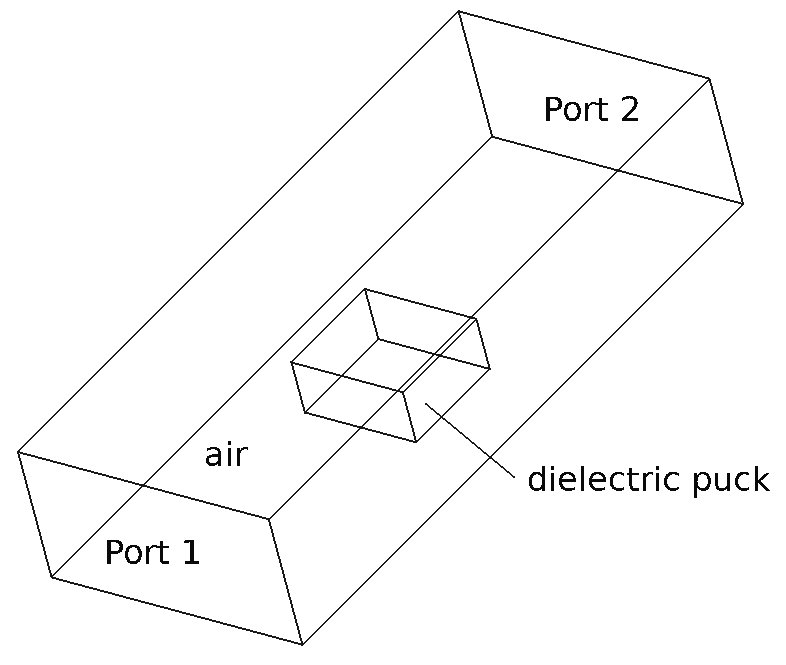
\includegraphics[width=0.4\textwidth]{../regression/OpenParEM3D/WR75/dielectric-loading_study/screenshots/loading_drawing}
  \caption{Drawing of a WR75 waveguide loaded by a dielectric puck with $\epsilon_r=6$.}
  \label{fig:loading_drawing}
\end{figure}

The longest mesh element in any of the materials is 0.39~$\lambda$ in length, so the structure is simulated \textit{without} adaptive mesh refinement using 4$^{\textnormal{th}}$-order elements.  The structure is simulated again with 
2$^{\textnormal{nd}}$-order elements \textit{with} adaptive mesh refinement at k$_o$b=0.26 with a relative tolerance of 0.001.  The results and comparisons are shown in Fig.~\ref{fig:loading_results}, where the agreement is excellent with the two curves overlaying each other.

For this accuracy study, the relative tolerance is set very tight at 0.001 for AMR, requiring 15 iterations for convergence and a final run time per frequency of about 42~s.  The results are essentially identical to those without AMR using 4$^{\textnormal{th}}$-order elements, but this simulation requires no time for adaptive refinement and about 7.5~s per frequency point.  This is a good example of how higher-order finite elements can simplify a setup and produce a much faster run time by eliminating the uncertainty of how tight to set the convergence tolerance for AMR.


\begin{figure}[H]
  \centering
  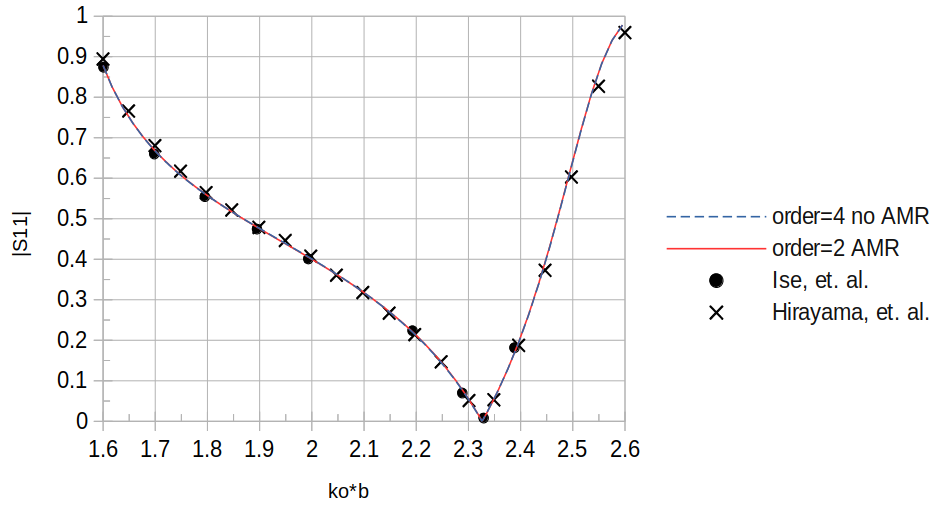
\includegraphics[width=0.6\textwidth]{../regression/OpenParEM3D/WR75/dielectric-loading_study/screenshots/loading_results}
  \caption{Results and comparisons to \cite{Ise} and \cite{Hirayama}.}
  \label{fig:loading_results}
\end{figure}

\subsection{Lossy Stripline}

The lossy stripline described in \cite{Simonovich} is simulated for comparison with the paper's simulation and measurement.
The project can be found in \texttt{regression/OpenParEM3D/stripline/Simonovich\_stripline\_study} of the OpenParEM distribution.
Using the file \texttt{regression/OpenParEM3D/stripline/Simonovich\_stripline\_study/builder.txt}, builder [see "OpenParEM2D\_User\_Manual.pdf"] is used to generate the structure..
A section just 1~mm long is constructed, and the results are multiplied by 6*25.4 to obtain results for a 6~in line.
The structure drawing is shown in Fig.~\ref{fig:stripline_drawing}, where extra physical detail is automatically added by builder to focus meshing on the trace edges.

The geo file from builder is meshed in gmsh with all default settings except that the mesh "Element size factor" is set to 1.8 to lower the mesh density, and the mesh is shown in Fig.~\ref{fig:stripline_mesh}.  Note that the mesh is quite dense even with the relaxation applied with the element size factor.  With a mesh this dense to begin with, low-order finite elements are suitable.

\begin{figure}[H]
  \centering
  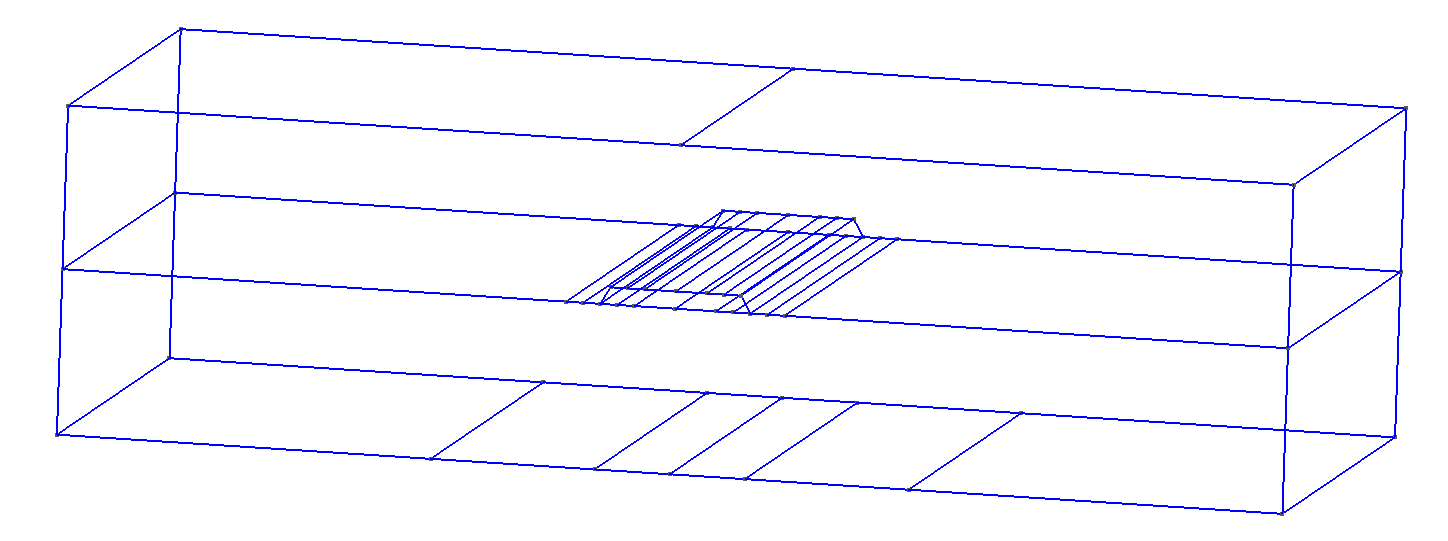
\includegraphics[width=0.5\textwidth]{../regression/OpenParEM3D/stripline/Simonovich_stripline_study/screenshots/stripline_drawing}
  \caption{Short 1~mm section of stripline as generated by builder.}
  \label{fig:stripline_drawing}
\end{figure}

\begin{figure}[H]
  \centering
  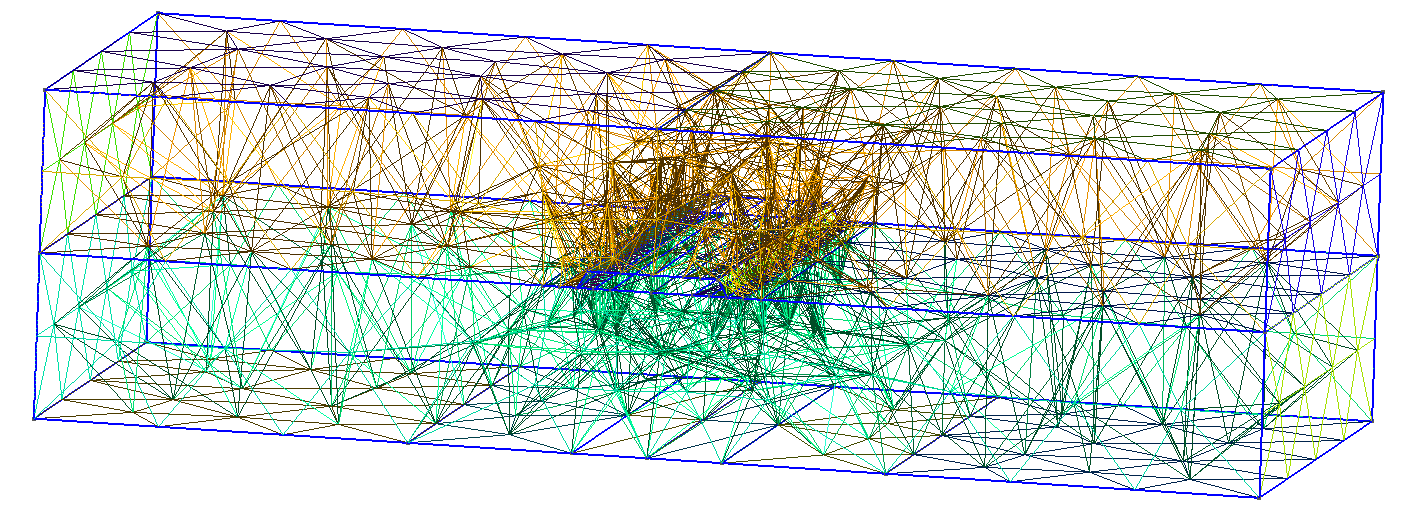
\includegraphics[width=0.5\textwidth]{../regression/OpenParEM3D/stripline/Simonovich_stripline_study/screenshots/stripline_mesh}
  \caption{Mesh of the short section of stripline.}
  \label{fig:stripline_mesh}
\end{figure}

The structure is simulated with 2$^{\textnormal{nd}}$-order elements with adaptive refinement at 50~GHz and convergence on the H-field metric using an absolute tolerance of $1\!\!\times\!\!10^{-8}$.  H-field convergence is used instead of S since the return loss continuously decreases as the accuracy improves.  The results and comparisons to the simulation and measurement in \cite{Simonovich} are shown in Fig.~\ref{fig:stripline_results}, and the agreement between both simulations and the measurement is excellent.

\begin{figure}[H]
  \centering
  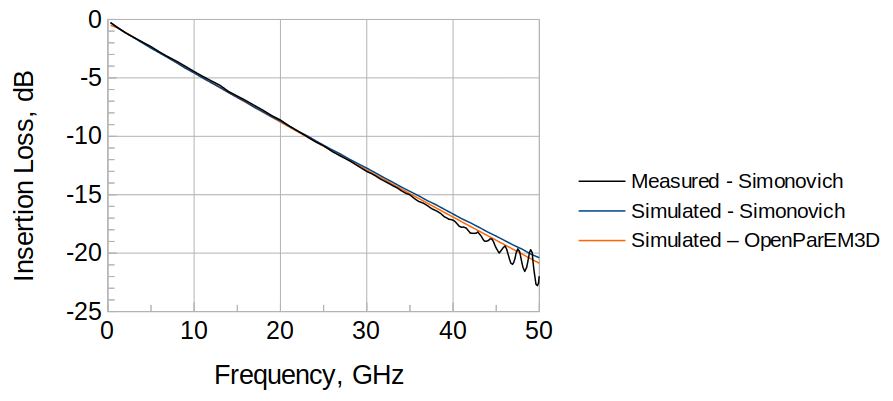
\includegraphics[width=0.7\textwidth]{../regression/OpenParEM3D/stripline/Simonovich_stripline_study/screenshots/stripline_results}
  \caption{Simulation results and comparisons to \cite{Simonovich}.}
  \label{fig:stripline_results}
\end{figure}

\subsection{Lossless WR90 Rectangular Waveguide}

A 100~mm-long straight section of lossless WR90 rectangular waveguide is simulated at 9~GHz to extremes to test accuracy, self-consistency, numerical noise floors, and adaptive mesh refinement.  The correct answers are known analytically as $|\textnormal{S11}|=0$, $|\textnormal{S21}|=1$, and S21 phase=-20.753057470156$^\circ$, so exact error calculations can be made.  Note that all of the regression suite cases using WR90 rectangular waveguide also make error calculations against analytical results.  The project can be found in the OpenParEM distribution in \texttt{regression/OpenParEM3D/WR90/straight\_study}.

The rectangular waveguide is set up in FreeCAD then minimally meshed with gmsh, and the resulting mesh is shown in Fig.~\ref{fig:WR90mesh}.  At 9~GHz this mesh is very coarse, with the longest tetrahedron edge 1.53$\lambda$ long.  Overall, the waveguide is 2.058$\lambda$ long as shown by the field plot in Fig.~\ref{fig:WR90ReEy}.

The waveguide is solved for finite element orders from 1 to 12.  Adaptive mesh refinement is allowed to proceed until  memory runs out.  MPI is run with 10 cores.  Larger numbers of cores are not possible with such a small initial mesh.

\begin{figure}[H]
  \centering
  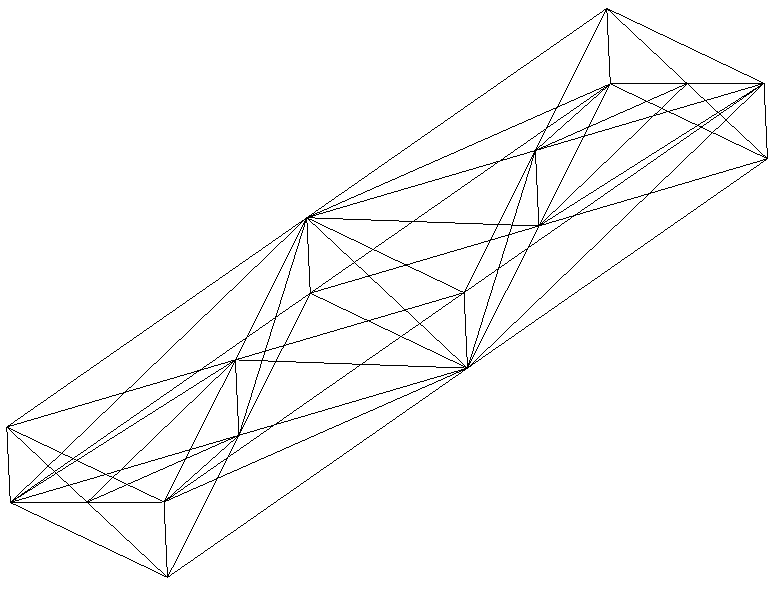
\includegraphics[width=0.4\textwidth]{../regression/OpenParEM3D/WR90/straight_study/screenshots/WR90mesh}
  \caption{Initial mesh for the 100 mm long WR90 rectangular waveguide.}
  \label{fig:WR90mesh}
\end{figure}

\begin{figure}[H]
  \centering
  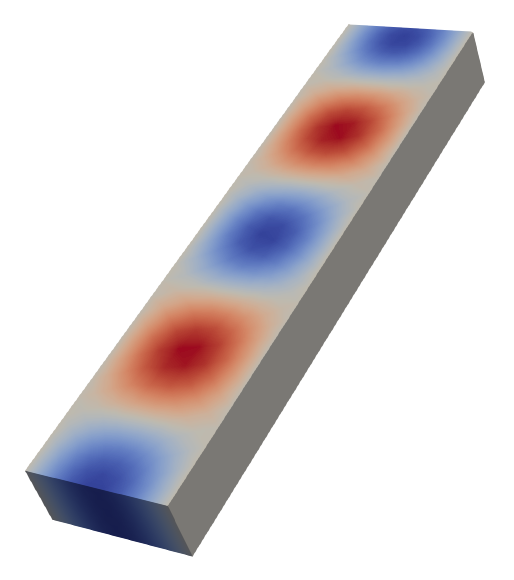
\includegraphics[width=0.3\textwidth]{../regression/OpenParEM3D/WR90/straight_study/screenshots/WR90ReEy}
  \caption{$\textnormal{Re}(E_y)$ at 9 GHz.}
  \label{fig:WR90ReEy}
\end{figure}

The S11 error is calculated as simply 20*log10(abs(S11)), and the results are plotted in Fig.~\ref{fig:S11Error} against the cumulative run time.  For finite element orders up to 10, adaptive refinement drives down the error, then the mesh because too dense for orders 11 and 12 and accuracy drops by a small amount. The effects of over-meshing for orders 11 and 12 appear in all other results in this study.  The results indicate a noise floor better than -160~dB.  For an error of 0.01\%, or -40~dB, finite element orders below 5 take some number of iterations to reach this accuracy target, with more iterations required for lower orders.  Also for this error target, the shortest run time is achieved with 5$^{\textnormal{th}}$-order finite elements with no adaptive refinement.

\begin{figure}[H]
  \centering
  \begin{subfigure}[t]{0.49\textwidth}
     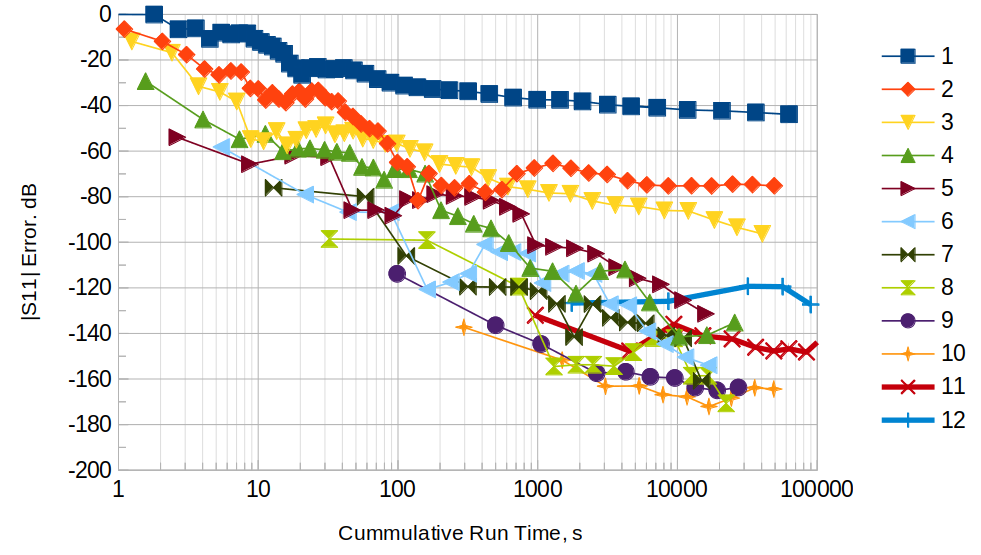
\includegraphics[width=1\linewidth]{../regression/OpenParEM3D/WR90/straight_study/screenshots/S11Error}
     \caption{Results.}
  \end{subfigure}
  \begin{subfigure}[t]{0.49\textwidth}
     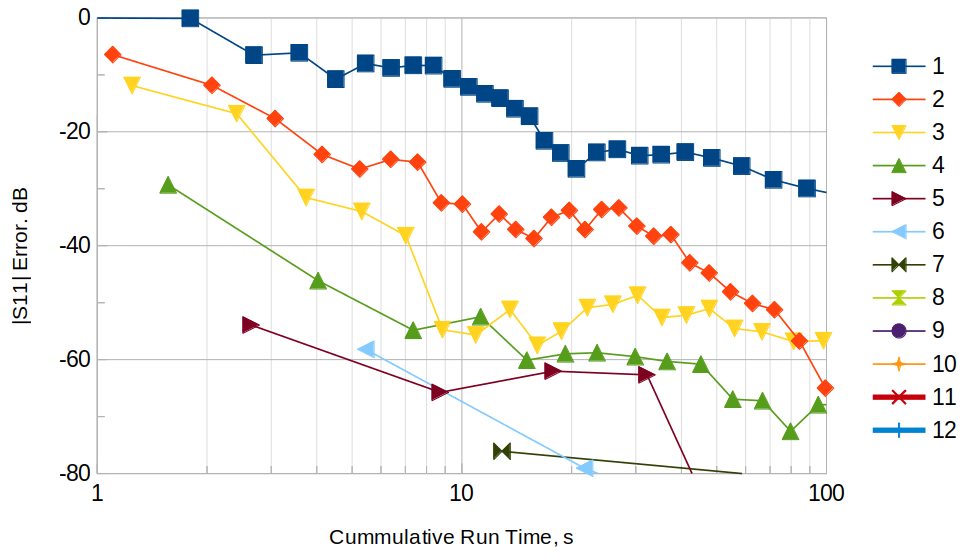
\includegraphics[width=1\linewidth]{../regression/OpenParEM3D/WR90/straight_study/screenshots/S11ErrorZoom}
     \caption{Zoom.}
  \end{subfigure}
  \caption{$|\textnormal{S11}|$ error.}
  \label{fig:S11Error}
\end{figure}

The S21 error is calculated as 20*log10(abs(1-abs(S21)), and the results are plotted in Fig.~\ref{fig:S21Error} against the cumulative run time.  The errors are lower than for S11 with a lower noise floor, and the adaptive refinement behavior is similar.

\begin{figure}[H]
  \centering
  \begin{subfigure}[t]{0.49\textwidth}
     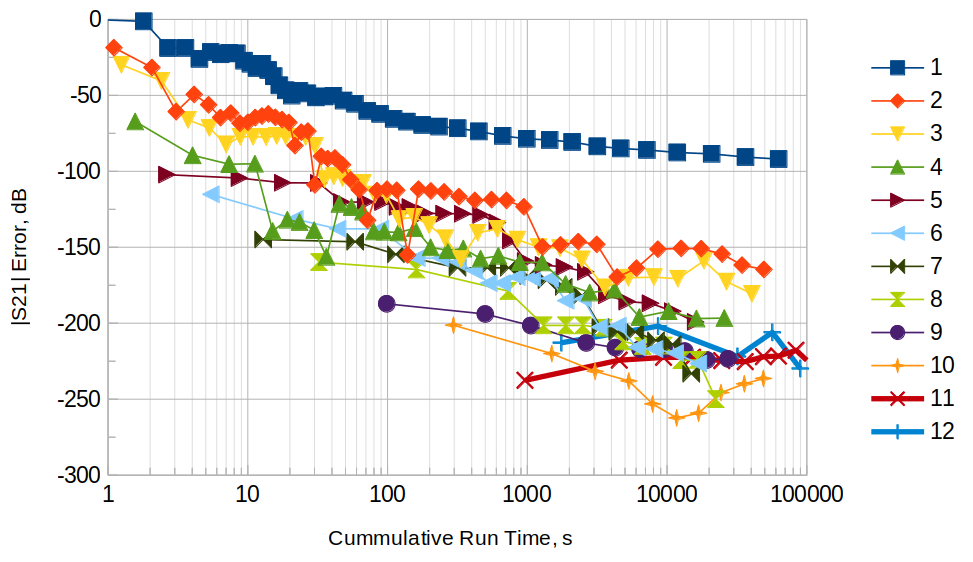
\includegraphics[width=1\linewidth]{../regression/OpenParEM3D/WR90/straight_study/screenshots/S21Error}
     \caption{Results.}
  \end{subfigure}
  \begin{subfigure}[t]{0.49\textwidth}
     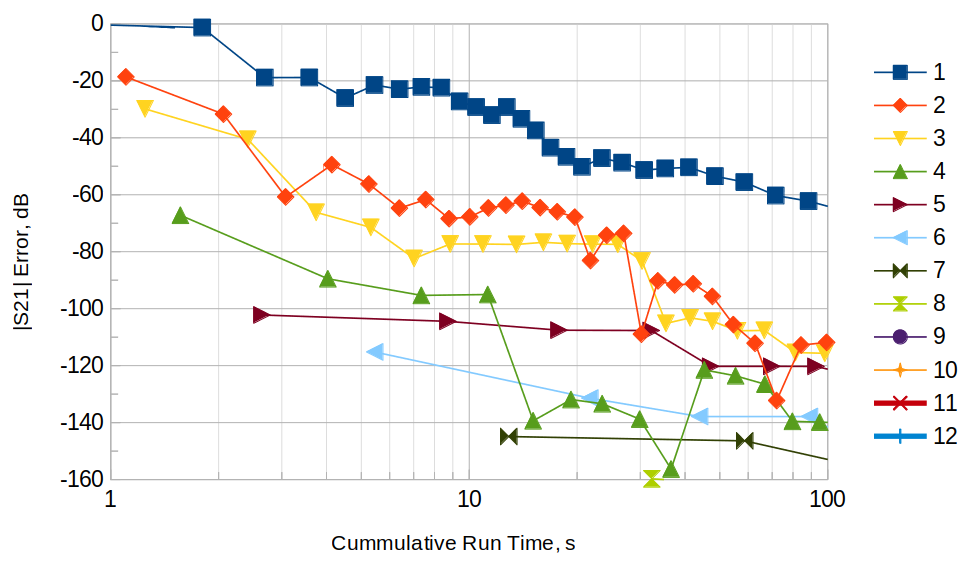
\includegraphics[width=1\linewidth]{../regression/OpenParEM3D/WR90/straight_study/screenshots/S21ErrorZoom}
     \caption{Zoom.}
  \end{subfigure}
  \caption{$|\textnormal{S21}|$ error.}
  \label{fig:S21Error}
\end{figure}

The phase shift error for S21 is calculated as 20*log10(abs((theta-arg(S21)/theta)), where \newline theta=-20.753057470156, and the results are plotted in Fig.~\ref{fig:PhaseShiftError}.  The errors are larger than for S11 but with a similar noise floor, and the adaptive refinement behavior is similar.  For a 0.01\% accuracy limit, 1$^{\textnormal{st}}$-order elements are not able to reach the target within a reasonable number of iterations.  Orders below 6 require adaptive refinement, and like for S11, higher orders require fewer iterations to reach a given level of error.  The shortest run time that achieves this accuracy target is 6$^{\textnormal{th}}$-order with no adaptive refinement. Considering both the S11 and phase shift results, for this problem, the 6$^{\textnormal{th}}$-order element is able to accurately model 1.53$\lambda$ long finite elements.

\begin{figure}[H]
  \centering
  \begin{subfigure}[t]{0.49\textwidth}
     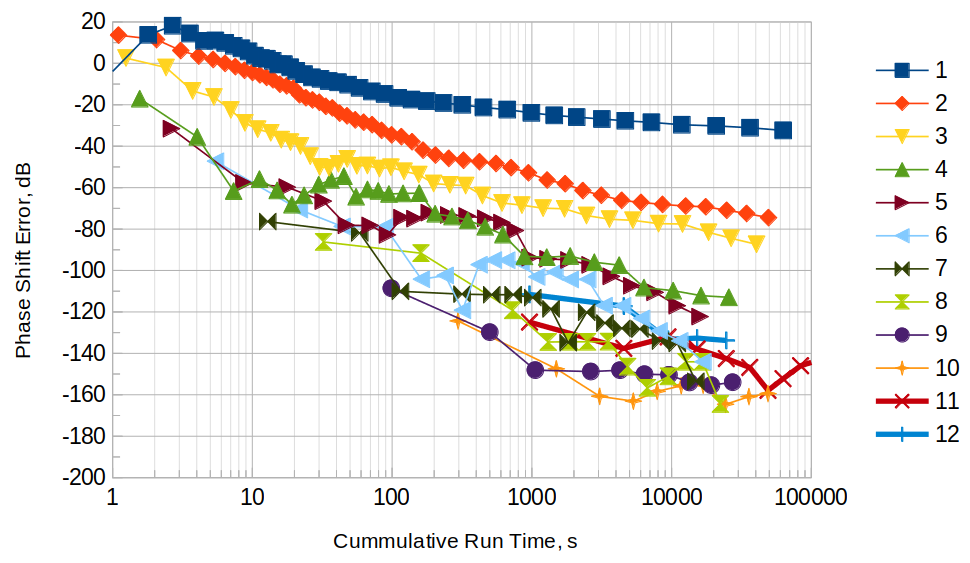
\includegraphics[width=1\linewidth]{../regression/OpenParEM3D/WR90/straight_study/screenshots/PhaseShiftError}
     \caption{Results.}
  \end{subfigure}
  \begin{subfigure}[t]{0.49\textwidth}
     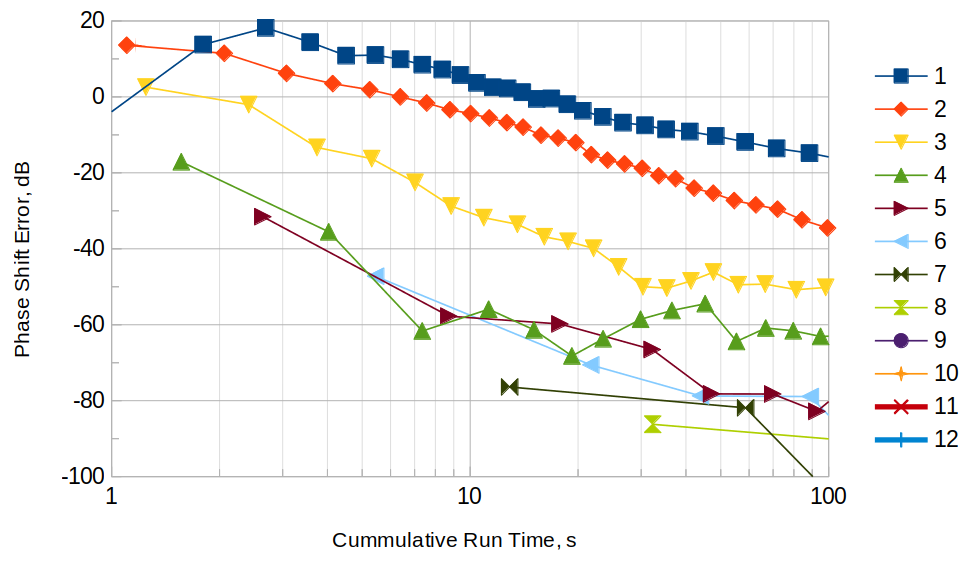
\includegraphics[width=1\linewidth]{../regression/OpenParEM3D/WR90/straight_study/screenshots/PhaseShiftErrorZoom}
     \caption{Zoom.}
  \end{subfigure}
  \caption{Phase shift error.}
  \label{fig:PhaseShiftError}
\end{figure}

Since this is a closed lossless problem, the total power in S11 and S21 must sum to 1.  The passivity error is calculated as 20*log10(abs(1-abs(S11)\string^2-abs(S21)\string^2)), and the results are shown in Fig.~\ref{fig:PassivityError}.  The passivity error is good for all orders with higher orders having lower errors and adaptive refinement generally improving errors for increasing iterations.  The passivity error improves as the accuracy improves.

\begin{figure}[H]
  \centering
  \begin{subfigure}[t]{0.49\textwidth}
     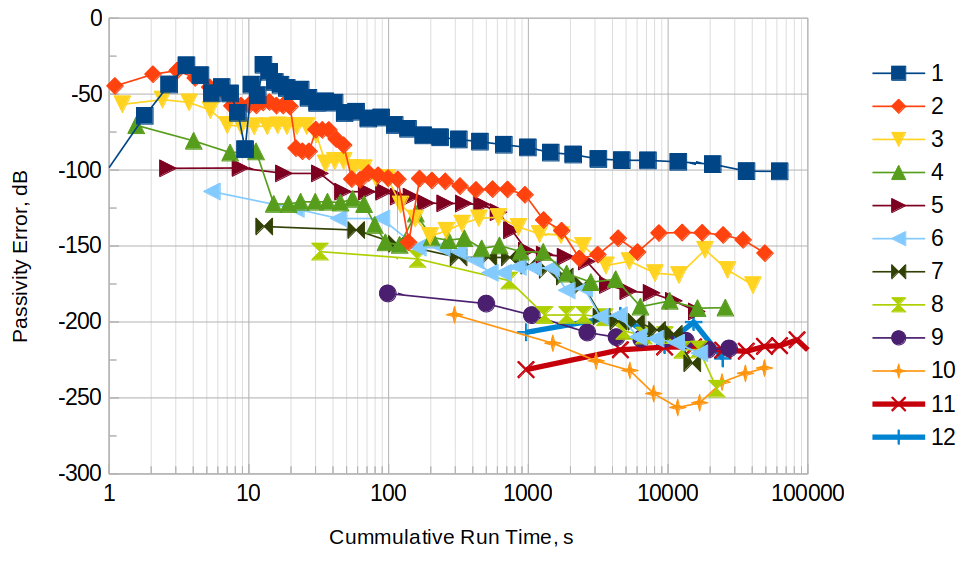
\includegraphics[width=1\linewidth]{../regression/OpenParEM3D/WR90/straight_study/screenshots/PassivityError}
     \caption{Results.}
  \end{subfigure}
  \begin{subfigure}[t]{0.49\textwidth}
     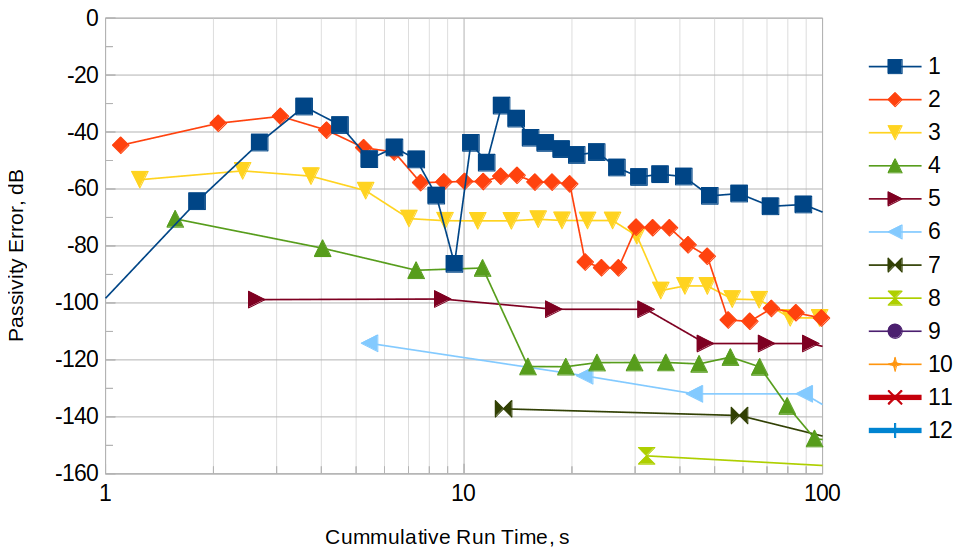
\includegraphics[width=1\linewidth]{../regression/OpenParEM3D/WR90/straight_study/screenshots/PassivityErrorZoom}
     \caption{Zoom.}
  \end{subfigure}
  \caption{Passivity error.}
  \label{fig:PassivityError}
\end{figure}

High-order finite elements offer some opportunity to skip adaptive mesh refinement.  In Fig.~\ref{fig:FirstIteration}, the S-parameter errors are plotted for just the initial iteration.  Again taking 0.01\% as an accuracy target, 6$^{\textnormal{th}}$-order and above finite elements can handle the 1.53$\lambda$ long elements in this problem.  Many of the regression suite test cases are solved without adaptive mesh refinement by using higher-order finite elements.

\begin{figure}[H]
  \centering
  \includegraphics[width=0.6\textwidth]{../regression/OpenParEM3D/WR90/straight_study/screenshots/FirstIteration}
  \caption{Errors for all finite element orders for just the first iteration.}
  \label{fig:FirstIteration}
\end{figure}

\subsection{Dipole Antenna}

A dipole antenna with balanced feed is simulated for the radiation pattern, directivity, gain, efficiency, and input impedance and compared to analytical results.  The antenna is shown in Fig.~\ref{fig:dipole_antenna}, where (a) shows the thin antenna with 60~$\mu m$ radius and 15~mm length modeled as a 12-sided cylinder, (b) shows a zoom of the balanced feed structure, and (c) shows the boxed structure plus concentric cylinders to produce a higher quality mesh.  The feed includes a dielectric filling (not shown) to enable tuning of the impedance and to break symmetry to ensure that the required mode is the dominant mode.  The default boundary condition is copper for the antenna and 1$^{\textnormal{st}}$-order radiation boundary conditions on the outer box.  The 15~mm length represents 1/2~$\lambda$ at 10~GHz, but it is well known that the resonant frequency pulls to a slightly lower frequency.

\begin{figure}[H]
  \centering
  \begin{subfigure}[t]{0.0125\textwidth}
     \includegraphics[width=1\linewidth]{../regression/OpenParEM3D/antenna/dipole_study/screenshots/dipole}
     \caption{Dipole with feed.}
  \end{subfigure}
  \hspace{1cm}
  \begin{subfigure}[t]{0.2\textwidth}
     \includegraphics[width=1\linewidth]{../regression/OpenParEM3D/antenna/dipole_study/screenshots/dipole_feed}
     \caption{Zoom of feed.}
  \end{subfigure}
  \hspace{1cm}
  \begin{subfigure}[t]{0.32\textwidth}
     \includegraphics[width=1\linewidth]{../regression/OpenParEM3D/antenna/dipole_study/screenshots/dipole_boxed}
     \caption{Complete drawing with concentric polygons and box.}
  \end{subfigure}
  \caption{Dipole antenna.}
  \label{fig:dipole_antenna}
\end{figure}

The mesh is generated using gmsh with default settings except that the "Element size factor" is set to 0.9 to improve the mesh quality and the "Max element size" is set to 0.0125 to limit the element size to about 1/2~$\lambda$ at 12~GHz. The limited mesh size enables finite elements with order 3 and higher to accurately model the fields in the transition and far-field regions without adaptive refinement.  Adaptive refinement is used to refine the fields in the feed structure and the near field region by limiting the extent of the refinement with \texttt{mesh.refinement.fraction} set to 0.001, and convergence takes 9 iterations using a relative convergence criteria of 0.001 on S at 12~GHz.

Using 4$^{\textnormal{th}}$-order finite elements with AMR at 12~GHz, the swept S-parameters are shown in Fig.~\ref{fig:dipole_S}, where the resonant frequency is about 9.38~GHz.  For a 15~mm length, the half-wavelength is 10~GHz, so the resonant frequency is pulled lower by 6.2\%.  The length/diameter ratio is 15~mm/60~$\mu m$=250, and interpolating Table~5-2 from \cite{Stutzman-Thiele} produces an estimated reduction in the resonant frequency of 3.8\%. The observed pulling is more than the estimate, but some additional pulling is expected due to the balanced port structure, which introduces capacitive coupling between the the two legs of the antenna due to the overlapping metal of the port box and due to the inductive side-feed that requires the currents to transition across the antenna and to establish a symmetric current profile.  The input impedance at 9.38~GHz is real and near the expected value of 73~$\Omega$.

\begin{figure}[H]
  \centering
  \includegraphics[width=0.6\textwidth]{../regression/OpenParEM3D/antenna/dipole_study/screenshots/dipole_S}
  \caption{Computed S11.}
  \label{fig:dipole_S}
\end{figure}

Post-processed results for far-field metrics are shown in Fig.~\ref{fig:dipole_gain}.  The analytical result for the directivity at resonance is 2.151, and the simulated value is 2.152 for a close match.  The efficiency peaks at 1.013, so there is a small passivity violation.  Re-simulating with the same mesh and 5$^{\textnormal{th}}$-order finite elements reduces the passivity violation to 1.0032, so violations are driven by accuracy.  The computed radiation pattern for $E_\theta$ is shown in Fig.~\ref{fig:dipole_pattern}, where (a) shows the full 3D patten with a clipping plane marked for the x-z plane, and (b) shows the 3D pattern clipped at the clipping plane.  This log plot shows the expected torus pattern for a dipole antenna.

The analytical result for $E_\theta$ is known from (2-10) in \cite{Stutzman-Thiele}.  The analytical and simulated results are shown in Fig.~\ref{fig:dipole_slice}, where the results overlay for a very high level of agreement.  Note that Fig.~\ref{fig:dipole_slice} is plotted on a linear scale, while Fig.~\ref{fig:dipole_pattern} is plotted on a log scale.

\begin{figure}[H]
  \centering
  \includegraphics[width=0.6\textwidth]{../regression/OpenParEM3D/antenna/dipole_study/screenshots/dipole_gain}
  \caption{Far-field metrics.}
  \label{fig:dipole_gain}
\end{figure}

\begin{figure}[H]
  \centering
  \begin{subfigure}[t]{0.33\textwidth}
     \includegraphics[width=1\linewidth]{../regression/OpenParEM3D/antenna/dipole_study/screenshots/dipole_pattern}
     \caption{$E_\theta$ with marked clipping plane.}
  \end{subfigure}
  \begin{subfigure}[t]{0.33\textwidth}
     \includegraphics[width=1\linewidth]{../regression/OpenParEM3D/antenna/dipole_study/screenshots/dipole_pattern_clip}
     \caption{$E_\theta$ clipped.}
  \end{subfigure}
  \caption{Far-field pattern for $E_\theta$.}
  \label{fig:dipole_pattern}
\end{figure}

\begin{figure}[H]
  \centering
  \includegraphics[width=0.8\textwidth]{../regression/OpenParEM3D/antenna/dipole_study/screenshots/dipole_slice}
  \caption{$E_\theta$ on the x-z slice comparing analytical and simulated results.}
  \label{fig:dipole_slice}
\end{figure}

\subsection{Patch Antenna}

The patch antenna from \cite{Mei} is simulated and compared to the paper's simulations and measurements.  The patch is shown in Fig.~\ref{fig:patch}, and the design consists of a rectangular metal patch on a conductor-backed F4B substrate with shorting vias tying the patch to the ground plane in four symmetric locations.  The patch is center-fed with 50$\Omega$ coax as shown in Fig.~\ref{fig:patch_detail}(a), and the boxed patch ready for simulation is shown in Fig.~\ref{fig:patch_detail}(b).  The model is constructed using the nominal dimensions and material parameters provided in the paper.

\begin{figure}[H]
  \centering
  \includegraphics[width=0.7\textwidth]{../regression/OpenParEM3D/antenna/patch_study/screenshots/patch}
  \caption{Patch antenna from \cite{Mei}.}
  \label{fig:patch}
\end{figure}

\begin{figure}[H]
  \centering
  \begin{subfigure}[t]{0.48\textwidth}
     \includegraphics[width=1\linewidth]{../regression/OpenParEM3D/antenna/patch_study/screenshots/patch_with_feed}
     \caption{Patch with coaxial feed.}
  \end{subfigure}
  \begin{subfigure}[t]{0.48\textwidth}
     \includegraphics[width=1\linewidth]{../regression/OpenParEM3D/antenna/patch_study/screenshots/patch_boxed}
     \caption{Boxed patch ready for simulation.}
  \end{subfigure}
  \caption{Wireframe details of the patch antenna.}
  \label{fig:patch_detail}
\end{figure}

At 6.4~GHz, the freespace wavelength is 46.88~mm.  In gmsh, the maximum triangle edge is limited to 24~mm, or about 1/2$\lambda$, and meshed with otherwise default settings.  Since the maximum element length in the transition area and the far field are no greater than about 1/2$\lambda$ in length, 3$^{\textnormal{rd}}$-order finite elements are used along with adaptive mesh refinement to focus refinement in the near field using \texttt{mesh.refinement.fraction} set to 0.001.  At 5.2~GHz, the box is 5.2$\lambda$ across.  AMR is set to refine at 6.4~GHz and to converge on S with a relative tolerance of 0.001.

The simulated isotropic gain for the 3D pattern at 5.8~GHz is shown in Fig.~\ref{fig:patch_3D_gain}, where (a) shows the main lobe and (b) shows the back lobes.  The range of gains from peak to peak-3dB are shown in (c) highlighted in red.

\begin{figure}[H]
  \centering
  \begin{subfigure}[t]{0.3\textwidth}
     \includegraphics[width=1\linewidth]{../regression/OpenParEM3D/antenna/patch_study/screenshots/patch_3D_gain}
     \caption{Main lobe.}
  \end{subfigure}
  \begin{subfigure}[t]{0.3\textwidth}
     \includegraphics[width=1\linewidth]{../regression/OpenParEM3D/antenna/patch_study/screenshots/patch_3D_gain_back_lobes}
     \caption{Back lobes.}
  \end{subfigure}
  \begin{subfigure}[t]{0.3\textwidth}
     \includegraphics[width=1\linewidth]{../regression/OpenParEM3D/antenna/patch_study/screenshots/patch_3D_3dB}
     \caption{Peak to peak-3dB gain shown in red.}
  \end{subfigure}
  \caption{Simulated 3D isotropic gain.}
  \label{fig:patch_3D_gain}
\end{figure}

The computed S11 results are shown vs. the measurements from \cite{Mei} in Fig.~\ref{fig:patch_S11}.  The agreement is quite good with a slightly lower simulated resonant frequency and deeper null.  Note that the simulation uses nominal datasheet values and does not include surface roughness.

\begin{figure}[H]
  \centering
  \includegraphics[width=0.6\textwidth]{../regression/OpenParEM3D/antenna/patch_study/screenshots/patch_S11}
  \caption{Simulation vs. measurement from \cite{Mei} for S11.}
  \label{fig:patch_S11}
\end{figure}

For examining the input impedance, S11 is processed to shift the reference plane from the port to the bottom of the ground plane.  S11 is then converted to Z and compared to the simulation results from \cite{Mei} in Fig.~\ref{fig:patch_impedance}. Agreement is good.

\begin{figure}[H]
  \centering
  \includegraphics[width=0.6\textwidth]{../regression/OpenParEM3D/antenna/patch_study/screenshots/patch_impedance}
  \caption{Simulation vs. simulation from \cite{Mei} for input impedance.}
  \label{fig:patch_impedance}
\end{figure}

The isotropic gain is computed and compared to the measurements from \cite{Mei} in Fig.~\ref{fig:patch_gain}.  The measured data is quite limited in bandwidth, but it is inferred that the simulations agree within a reasonable 0.5~dBi.

\begin{figure}[H]
  \centering
  \includegraphics[width=0.7\textwidth]{../regression/OpenParEM3D/antenna/patch_study/screenshots/patch_gain}
  \caption{Simulation vs. measurement from \cite{Mei} for isotropic gain.}
  \label{fig:patch_gain}
\end{figure}

For the radiation pattern for $E_{\theta}$, simulations and measurements from \cite{Mei} are compared in Fig.~\ref{fig:patch_xz_pattern}.  The measured pattern seems to have a small alignment flaw, but generally, the simulation and measurement have very good agreement.

\begin{figure}[H]
  \centering
  \includegraphics[width=0.7\textwidth]{../regression/OpenParEM3D/antenna/patch_study/screenshots/patch_xz_pattern}
  \caption{Simulation vs. measurement from \cite{Mei} for $E_{\theta}$ in the x-z plane.}
  \label{fig:patch_xz_pattern}
\end{figure}





\begin{thebibliography}{unsrt}

\bibitem{MFEM} R. Anderson, J. Andrej, A. Barker, J. Bramwell, J.-S. Camier, J. Cerveny, V. Dobrev, Y. Dudouit, A. Fisher, Tz. Kolev, W. Pazner, M. Stowell, V. Tomov, I. Akkerman, J. Dahm, D. Medina, and S. Zampini, "MFEM: A modular finite element methods library", \textit{Computers and Mathematics with Applications}, vol. 81, 2021, pp. 42-74.

\bibitem{MFEMweb} \verb+https://mfem.org+

\bibitem{PETSc} \verb+https://petsc.org+

\bibitem{Balanis} Constantine Balanis, \textit{Advanced Engineering Electromagnetics}, John Wiley and Sons, 1989, pp. 288-289.

\bibitem{ParaView} \verb+https://www.paraview.org/+

\bibitem{Young} Brian Young, \textit{Digital Signal Integrity: Modeling and Simulation with Interconnects and Packages}, Prentice-Hall PTR, 2001.

\bibitem{Meyer} Petrie Meyer and David S. Prinsloo, "Generalized multimode scattering parameter and antenna far-field conversions," \textit{IEEE Trans. Antennas and Propagation}, vol. 63, no. 11, Nov. 2015, pp. 4818-4826.

\bibitem{Weng} Wei-Chung Weng, “Design and optimization of compact microstrip wideband bandpass filter using Taguchi’s method,” \textit{IEEE Open Access Journal}, vol. 10, 2022, pp. 107242-107249.

\bibitem{FreeCAD} \verb+https://www.freecad.org/+

\bibitem{gmsh} C. Geuzaine and J.-F. Remacle, "Gmsh: a three-dimensional finite element mesh generator with built-in pre- and post-processing facilities," \textit{International Journal for Numerical Methods in Engineering}, 79(11), pp. 1309-1331, 2009.

\bibitem{gmshweb} \verb+https://gmsh.info/+

\bibitem{Wong} Kin-Lu Wong, Chih-Hsien Wu, and Saou-Wen Su, "Ultrawide-band square planar metal-plate monopole antenna with a trident-shaped feeding strip," \textit{IEEE Trans. Antennas and Propagation}, vol. 53, no. 4, April 2005, pp. 1262-1269.

\bibitem{Wang} J.-S. Wang, and R. Mittra, “Finite element analysis of MMIC structures and electronic packages using absorbing boundary conditions,” \textit{IEEE Trans. Microwave Theory and Techniques}, vol. 42, no. 3, March 1994, pp. 441-449.

\bibitem{Hirayama} K. Hirayama, Md. Alam, Y. Hayashi, and M. Koshiba, “Vector finite element method with mixed-interpolation-type triangular-prism element for waveguide discontinuities,” \textit{IEEE Trans. Microwave Theory and Techniques}, vol. 42, no. 12, Dec. 1994, pp. 2311-2316.

\bibitem{Alessandri} F. Alessandri, M. Dionigi, and R. Rorrentino, “Rigorous analysis of compensated E-plane junctions in rectangular waveguide,” \textit{1995 IEEE MTT-S Digest}, pp. 987-990.

\bibitem{Ise} K. Ise, K. Inoue, and M. Koshiba, “Three-dimensional finite-element solution of dielectric scattering obstacles in a rectangular waveguide,” \textit{IEEE Trans. Microwave Theory and Techniques}, vol. 38, no. 9, Sept. 1990, pp. 1352-1359.

\bibitem{Simonovich} Lambert Simonovich, “A practical method to model effective permittivity and phase delay due to conductor surface roughness”, \textit{2017 DesignCon}.

\bibitem{Stutzman-Thiele} Warren L. Stutzman and Gary A. Thiele, \textit{Antenna Theory and Design}, John Wiley and Sons, 1981.

\bibitem{Mei} Peng Mei, Shuai Zhang, Xian Qi Lin, and Gert Fr\o lund Pedersen, "A low-profile patch antenna with monopole-like radiation patterns," \textit{2019 IEEE-APS Topical Conference on Antennas and Propagation in Wireless Communications (APWC)}, pp. 66-68.

\end{thebibliography}

\end{document}
